% Ensure that you compile using XeLaTeX !!! PDFTex has problems with some of the packages used
\documentclass[12pt]{article}
\setlength\parindent{0pt}

\usepackage{parskip}
\usepackage[margin=0.5in]{geometry}
\usepackage{fullpage}
\usepackage{moresize}
\usepackage{graphicx}
\usepackage{caption}
\usepackage{subcaption}
\usepackage{float}
\usepackage{xcolor}
\usepackage{soul}
\usepackage{fontspec}
\setmainfont{Doulos SIL}

\begin{document}

\begin{center}
\textbf{{\color{violet}{\HUGE ALL QUESTIONS\\}}}

\textbf{{\color{violet}{\HUGE BY TOPIC\\}}}

\end{center}
\newpage

\textbf{\underline{\huge Other (pre-midterm) / easy\\}}

~\\

{\large Question 1} (completed 20200915) - Source: Quiz 1, Question 7\\

Is this sentence prescriptive or descriptive? Explain why.\\

People speaking standard North American English use <doesn't> with the pronoun <he>, as in ``He doesn't seem concerned today.''


~\\
INSTRUCTOR NOTES: 


~\\

{\large Question 2} (completed 20200915) - Source: Quiz 1, Question 7\\

Is this sentence prescriptive or descriptive? Explain why.\\

People who say <ain't> may suffer some negative social consequences, because many speakers of English associate <ain't> with a lack of education.


~\\
INSTRUCTOR NOTES: 


~\\

{\large Question 3} (completed 20200915) - Source: Quiz 1, Question 7\\

Is this sentence prescriptive or descriptive? Explain why.\\

In casual styles of speaking, English speakers frequently end sentences with prepositions, but ending sentences with prepositions is avoided in formal styles.


~\\
INSTRUCTOR NOTES: 


~\\

{\large Question 4} (completed 20200915) - Source: Quiz 1, Question 7\\

Is this sentence prescriptive or descriptive? Explain why.\\

Saying ``Between you and me'' is correct; saying ``Between you and I'' is ungrammatical.


~\\
INSTRUCTOR NOTES: 


~\\

{\large Question 5} (completed 20200918) - Source: Week 2 Handout, Part I, Question 5\\

Is this question about phonetics or phonology, and why? (To be clear: you do NOT need to answer the question itself -- just tell me whether it's a question about phonetics or phonology.)\\

Try producing an {[s]} for a long time ({[sssssssssssssss]}). How long can you let it out? What do you have to do physically to make it last longer?


~\\
INSTRUCTOR NOTES: phonetics


~\\

{\large Question 6} (completed 20200918) - Source: Week 2 Handout, Part I, Question 6\\

Is this question about phonetics or phonology, and why? (To be clear: you do NOT need to answer the question itself -- just tell me whether it's a question about phonetics or phonology.)\\

How would you describe the differences between an {[s]} and an {[f]}? what about between {[s]} and {[t]}? or between {[s]} and {[z]}? Think about how they sound, how it feels to produce them, how they look when you see other people producing them, etc.


~\\
INSTRUCTOR NOTES: phonetics


~\\

{\large Question 7} (completed 20200918) - Source: Week 2 Handout, Part I, Question 9\\

Is this question about phonetics or phonology, and why? (To be clear: you do NOT need to answer the question itself -- just tell me whether it's a question about phonetics or phonology.)\\

Which is louder, the vowel sound {[ah]} or the consonant sound {[f]}? Why do you think that is?


~\\
INSTRUCTOR NOTES: phonetics


~\\

{\large Question 8} (completed 20200918) - Source: Week 2 Handout, Part I, Question 10\\

Is this question about phonetics or phonology, and why? (To be clear: you do NOT need to answer the question itself -- just tell me whether it's a question about phonetics or phonology.)\\

Consider the following pairs of words. In each pair, if you had to pick one of the two words for the name of a new product in English, which would you pick, and why? \begin{itemize} \item <bnick> or <blick> \item <rmagl> or <glarm> \item <ngitf> or <sfing> \end{itemize}


~\\
INSTRUCTOR NOTES: phonology


~\\

{\large Question 9} (completed 20201001) - Source: Quiz 3, Question 14\\

Does the morpheme ‘eye’ occur in this word? Why or why not?\\

<Eiffel> (as in Eiffel Tower)


~\\
INSTRUCTOR NOTES: 


~\\

{\large Question 10} (completed 20201001) - Source: Quiz 3, Question 14\\

Does the morpheme ‘eye’ occur in this word? Why or why not?\\

<disobeyed>


~\\
INSTRUCTOR NOTES: 


~\\

{\large Question 11} (completed 20201001) - Source: Quiz 3, Question 14\\

Does the morpheme ‘eye’ occur in this word? Why or why not?\\

<eyeglasses>


~\\
INSTRUCTOR NOTES: 


~\\

{\large Question 12} (completed 20201001) - Source: Quiz 3, Question 14\\

Does the morpheme ‘eye’ occur in this word? Why or why not?\\

<island>


~\\
INSTRUCTOR NOTES: 


~\\

{\large Question 13} (completed 20201001) - Source: Quiz 3, Question 14\\

Does the morpheme ‘eye’ occur in this word? Why or why not?\\

<eyes>


~\\
INSTRUCTOR NOTES: 


~\\

{\large Question 14} (completed 20201001) - Source: Quiz 3, Question 14\\

Does the morpheme ‘eye’ occur in this word? Why or why not?\\

<eyeful>


~\\
INSTRUCTOR NOTES: 


~\\

{\large Question 15} (completed 20201001) - Source: Quiz 3, Question 14\\

Does the morpheme ‘eye’ occur in this word? Why or why not?\\

<spyglass>


~\\
INSTRUCTOR NOTES: 


~\\

{\large Question 16} (completed -nodate-) - Source: \\

Explain why the following statement is false.\\

A phoneme can be defined as the smallest unit of sound that has a meaning.


~\\
INSTRUCTOR NOTES: 


\newpage\textbf{\underline{\huge Other (pre-midterm) / medium\\}}

~\\

{\large Question 1} (completed 20200918) - Source: Week 2 Handout, Part I, Question 1\\

Is this question about phonetics or phonology, and why? (To be clear: you do NOT need to answer the question itself -- just tell me whether it's a question about phonetics or phonology.)\\

What do you think the difference is between vowels and consonants?


~\\
INSTRUCTOR NOTES: 


~\\

{\large Question 2} (completed 20200918) - Source: Week 2 Handout, Part I, Question 7\\

Is this question about phonetics or phonology, and why? (To be clear: you do NOT need to answer the question itself -- just tell me whether it's a question about phonetics or phonology.)\\

How would you describe the difference between the vowel in the word <heat> and the vowel in the word <hat>?


~\\
INSTRUCTOR NOTES: phonetics


~\\

{\large Question 3} (completed 20200918) - Source: Week 2 Handout, Part I, Question 8\\

Is this question about phonetics or phonology, and why? (To be clear: you do NOT need to answer the question itself -- just tell me whether it's a question about phonetics or phonology.)\\

Consider the following two words from American Sign Language. The first one means LUCKY, while the second means SMART. How would you describe the difference between the ``pronunciation'' (articulation) of these two words? Note that in each case, the image to the left is the starting position of the sign, while the one to the right is the ending position.

\begin{figure}[H]
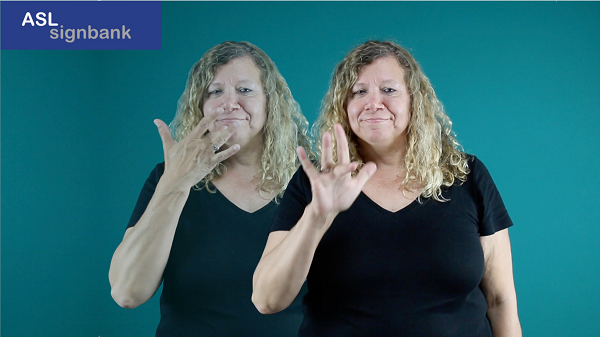
\includegraphics{../images/asl_lucky.png}
\end{figure}
\begin{figure}[H]
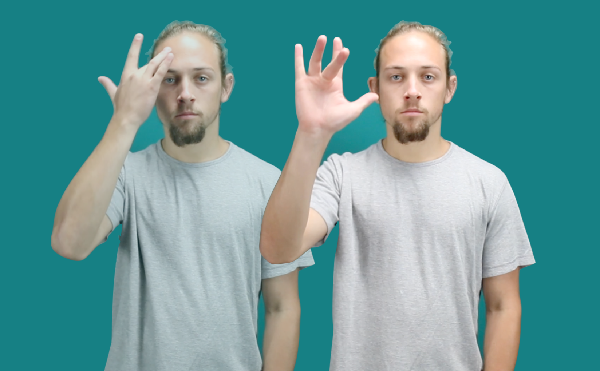
\includegraphics{../images/asl_smart.png}
\end{figure}

~\\
INSTRUCTOR NOTES: phonetics


~\\

{\large Question 4} (completed 20200918) - Source: Week 2 Handout, Part I, Question 12\\

Is this question about phonetics or phonology, and why? (To be clear: you do NOT need to answer the question itself -- just tell me whether it's a question about phonetics or phonology.)\\

What’s the difference in sound between the words <but> and <cut> in English? Is that the same difference as between <bit> and <kit>? Why or why not?


~\\
INSTRUCTOR NOTES: both


~\\

{\large Question 5} (completed 20201002) - Source: Week 4 Handout, Part II, Question 2(iii)\\

Explain how you would figure out the meaning of this Swahili word. (To be clear: you do NOT need to give me the meaning itself -- just explain the process of figuring it out.)\\

{[alikusumbua]}

\begin{figure}[H]
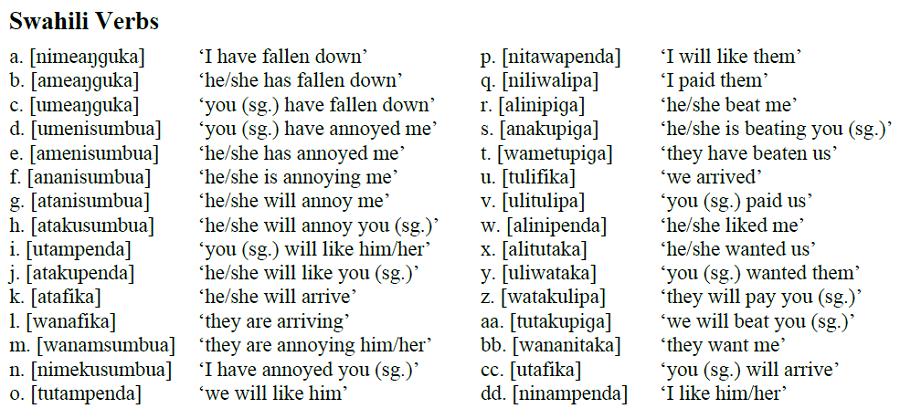
\includegraphics{../images/swahiliverbs.png}
\end{figure}

~\\
INSTRUCTOR NOTES: (he/she annoyed you (sg.))


~\\

{\large Question 6} (completed 20201002) - Source: Week 4 Handout, Part II, Question 2(iii)\\

Explain how you would figure out the meaning of this Swahili word. (To be clear: you do NOT need to give me the meaning itself -- just explain the process of figuring it out.)\\

{[tunampenda]}

\begin{figure}[H]
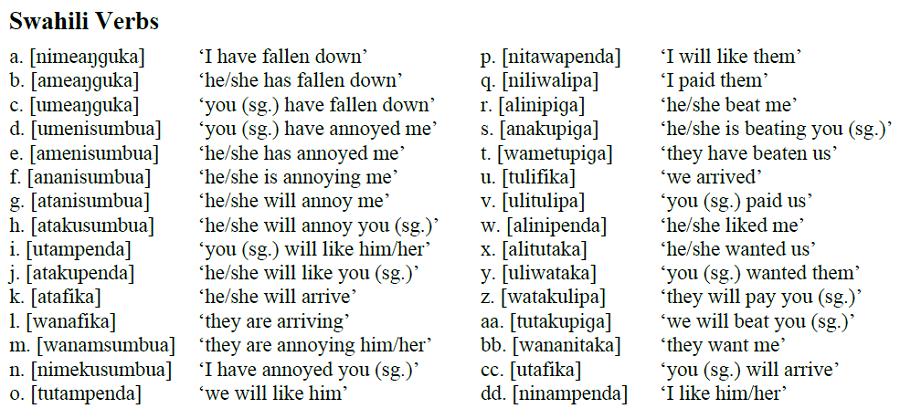
\includegraphics{../images/swahiliverbs.png}
\end{figure}

~\\
INSTRUCTOR NOTES: (we like him/her)


~\\

{\large Question 7} (completed 20201002) - Source: Week 4 Handout, Part II, Question 2(iii)\\

Explain how you would figure out the meaning of this Swahili word. (To be clear: you do NOT need to give me the meaning itself -- just explain the process of figuring it out.)\\

{[umefika]}

\begin{figure}[H]
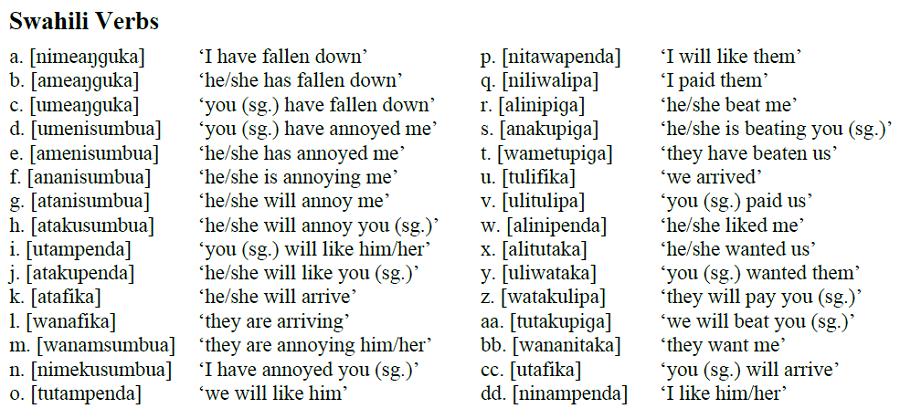
\includegraphics{../images/swahiliverbs.png}
\end{figure}

~\\
INSTRUCTOR NOTES: (you (sg.) have arrived)


~\\

{\large Question 8} (completed 20201002) - Source: Week 4 Handout, Part II, Question 2(iii)\\

Explain how you would figure out the meaning of this Swahili word. (To be clear: you do NOT need to give me the meaning itself -- just explain the process of figuring it out.)\\

{[watanipiɡa]}

\begin{figure}[H]
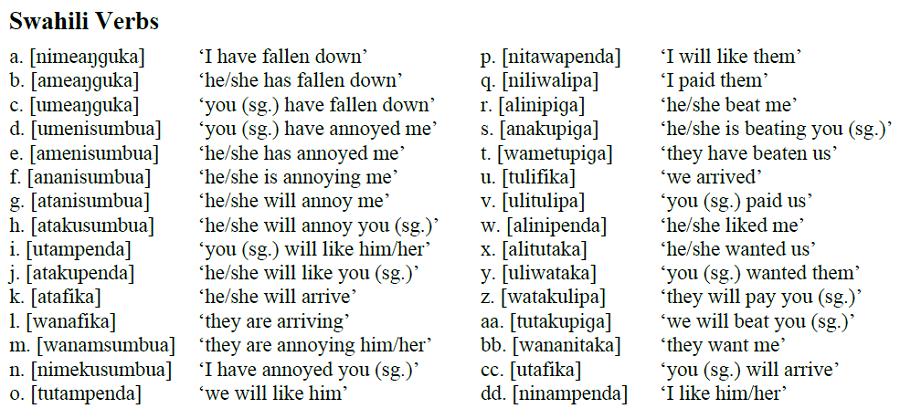
\includegraphics{../images/swahiliverbs.png}
\end{figure}

~\\
INSTRUCTOR NOTES: (they will beat me)


~\\

{\large Question 9} (completed 20201002) - Source: Week 4 Handout, Part II, Question 2(iv)\\

Explain how you would figure out the Swahili word for this English gloss. (To be clear: you do NOT need to give me the Swahili form itself -- just explain the process of figuring it out.)\\

‘I like you (sg.).’

\begin{figure}[H]
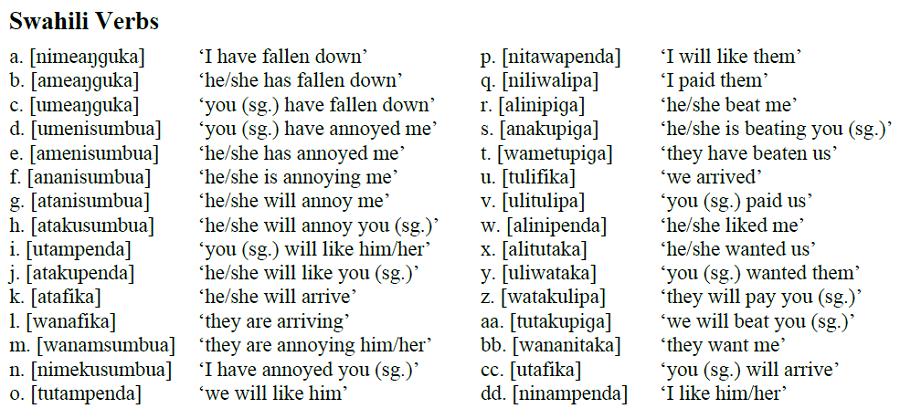
\includegraphics{../images/swahiliverbs.png}
\end{figure}

~\\
INSTRUCTOR NOTES: ([ninakupenda])


~\\

{\large Question 10} (completed 20201002) - Source: Week 4 Handout, Part II, Question 2(iv)\\

Explain how you would figure out the Swahili word for this English gloss. (To be clear: you do NOT need to give me the Swahili form itself -- just explain the process of figuring it out.)\\

‘We have fallen down.’

\begin{figure}[H]
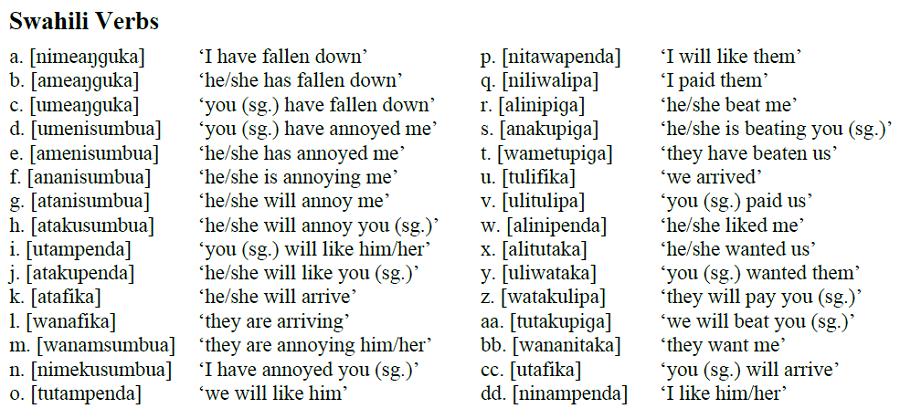
\includegraphics{../images/swahiliverbs.png}
\end{figure}

~\\
INSTRUCTOR NOTES: ([tumeaŋɡuka])


~\\

{\large Question 11} (completed 20201002) - Source: Week 4 Handout, Part II, Question 2(iv)\\

Explain how you would figure out the Swahili word for this English gloss. (To be clear: you do NOT need to give me the Swahili form itself -- just explain the process of figuring it out.)\\

‘She will beat us.’

\begin{figure}[H]
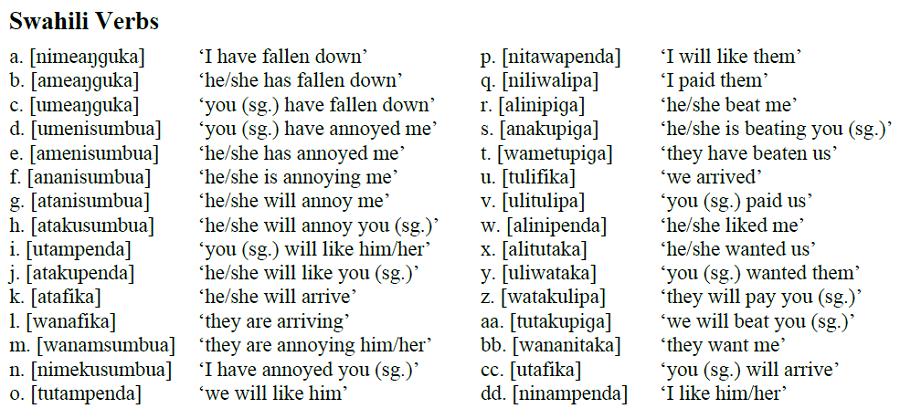
\includegraphics{../images/swahiliverbs.png}
\end{figure}

~\\
INSTRUCTOR NOTES: ([atatupiga])


~\\

{\large Question 12} (completed 20201002) - Source: Week 4 Handout, Part II, Question 2(iv)\\

Explain how you would figure out the Swahili word for this English gloss. (To be clear: you do NOT need to give me the Swahili form itself -- just explain the process of figuring it out.)\\

‘You (sg.) are annoying me.’

\begin{figure}[H]
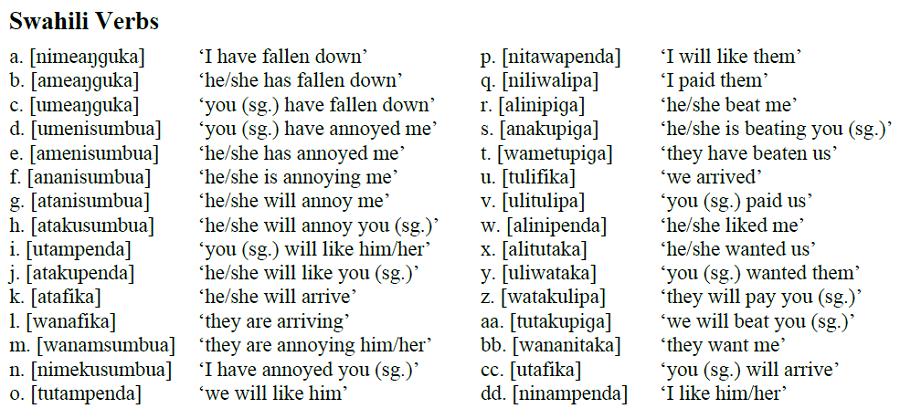
\includegraphics{../images/swahiliverbs.png}
\end{figure}

~\\
INSTRUCTOR NOTES: ([unanisumbua])


~\\

{\large Question 13} (completed 20201002) - Source: Week 4 Handout, Part II, Question 2(iv)\\

Explain how you would figure out the Swahili word for this English gloss. (To be clear: you do NOT need to give me the Swahili form itself -- just explain the process of figuring it out.)\\

‘They will pay him.’

\begin{figure}[H]
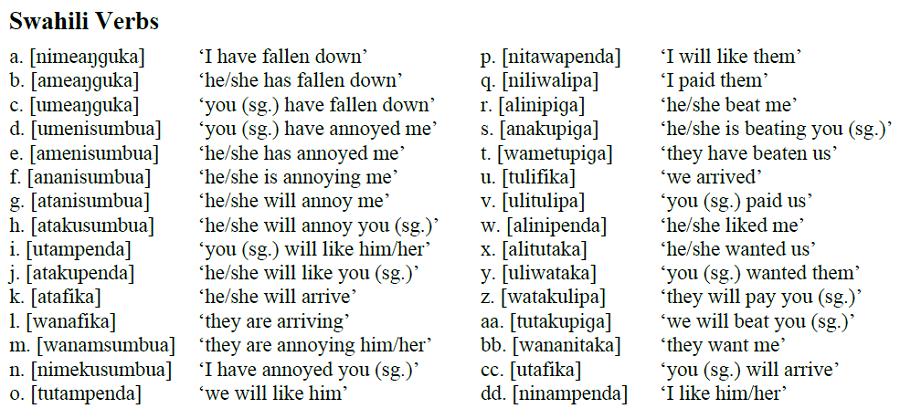
\includegraphics{../images/swahiliverbs.png}
\end{figure}

~\\
INSTRUCTOR NOTES: ([watamlipa])


~\\

{\large Question 14} (completed 20201002) - Source: Week 4 Handout, Part II, Question 2(iv)\\

Explain how you would figure out the Swahili word for this English gloss. (To be clear: you do NOT need to give me the Swahili form itself -- just explain the process of figuring it out.)\\

‘I wanted them.’

\begin{figure}[H]
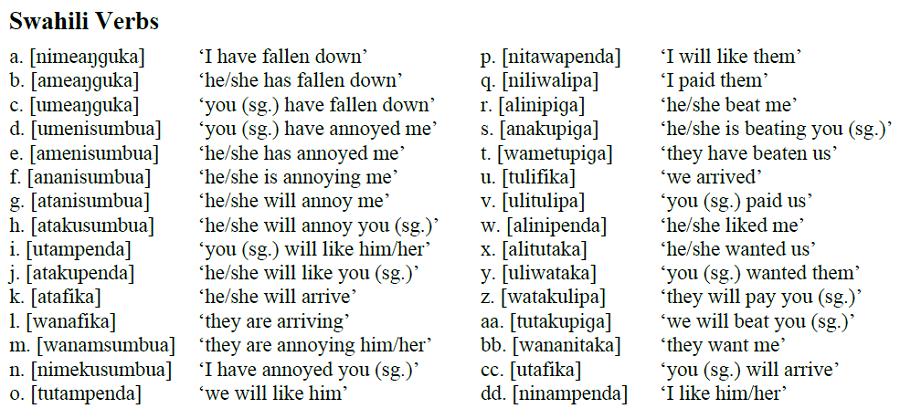
\includegraphics{../images/swahiliverbs.png}
\end{figure}

~\\
INSTRUCTOR NOTES: ([niliwataka])


~\\

{\large Question 15} (completed 20201001) - Source: Week 4 Handout, Part II, Question 3\\

Explain how you would figure out what the Luiseño form is for the morpheme whose meaning is given below. (To be clear: you do NOT need to give me the form itself -- just explain the process of figuring it out.)\\

‘first person singular subject’ (‘I’)

\begin{figure}[H]
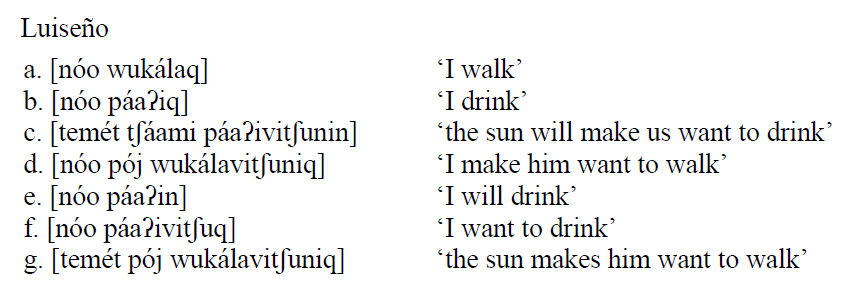
\includegraphics{../images/luiseno.png}
\end{figure}

~\\
INSTRUCTOR NOTES: ([nóo])


~\\

{\large Question 16} (completed 20201001) - Source: Week 4 Handout, Part II, Question 3\\

Explain how you would figure out what the Luiseño form is for the morpheme whose meaning is given below. (To be clear: you do NOT need to give me the form itself -- just explain the process of figuring it out.)\\

‘first person plural object’ (‘us’)

\begin{figure}[H]
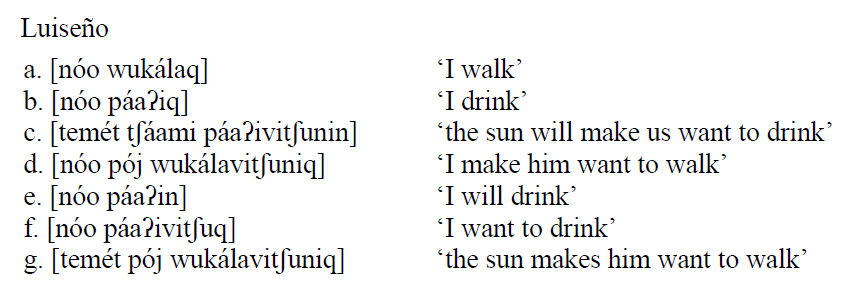
\includegraphics{../images/luiseno.png}
\end{figure}

~\\
INSTRUCTOR NOTES: ([tʃáami])


~\\

{\large Question 17} (completed 20201001) - Source: Week 4 Handout, Part II, Question 3\\

Explain how you would figure out what the Luiseño form is for the morpheme whose meaning is given below. (To be clear: you do NOT need to give me the form itself -- just explain the process of figuring it out.)\\

‘walk’

\begin{figure}[H]
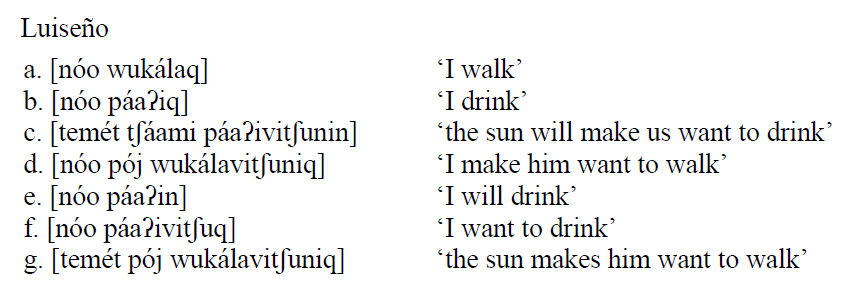
\includegraphics{../images/luiseno.png}
\end{figure}

~\\
INSTRUCTOR NOTES: ([wukála])


~\\

{\large Question 18} (completed 20201001) - Source: Week 4 Handout, Part II, Question 3\\

Explain how you would figure out what the Luiseño form is for the morpheme whose meaning is given below. (To be clear: you do NOT need to give me the form itself -- just explain the process of figuring it out.)\\

‘want’

\begin{figure}[H]
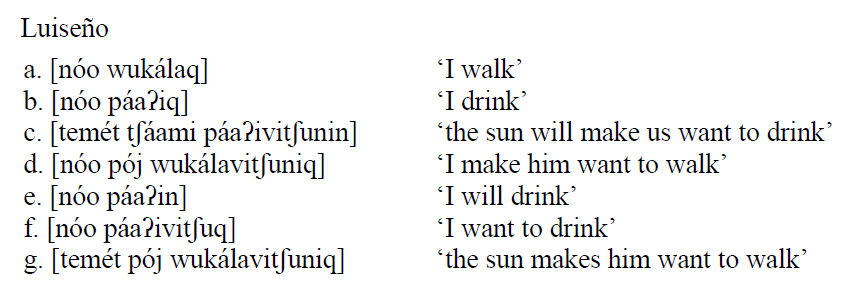
\includegraphics{../images/luiseno.png}
\end{figure}

~\\
INSTRUCTOR NOTES: ([vitʃu])


~\\

{\large Question 19} (completed 20201001) - Source: Week 4 Handout, Part II, Question 3\\

Explain how you would figure out what the Luiseño form is for the morpheme whose meaning is given below. (To be clear: you do NOT need to give me the form itself -- just explain the process of figuring it out.)\\

‘present tense’

\begin{figure}[H]
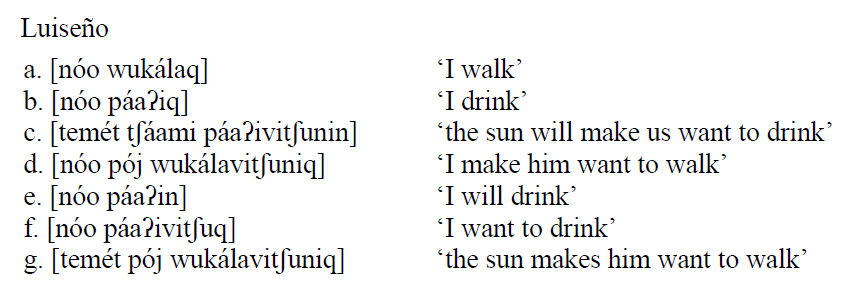
\includegraphics{../images/luiseno.png}
\end{figure}

~\\
INSTRUCTOR NOTES: ([q])


~\\

{\large Question 20} (completed 20201001) - Source: Week 4 Handout, Part II, Question 3\\

Explain how you would figure out what the Luiseño form is for the morpheme whose meaning is given below. (To be clear: you do NOT need to give me the form itself -- just explain the process of figuring it out.)\\

‘third person masc. object’ (‘him’)

\begin{figure}[H]
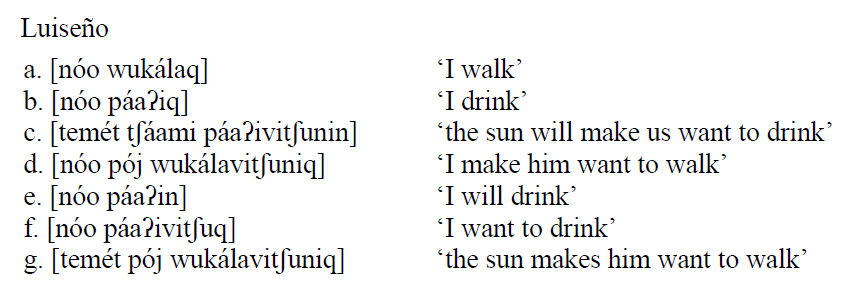
\includegraphics{../images/luiseno.png}
\end{figure}

~\\
INSTRUCTOR NOTES: ([pój])


~\\

{\large Question 21} (completed 20201001) - Source: Week 4 Handout, Part II, Question 3\\

Explain how you would figure out what the Luiseño form is for the morpheme whose meaning is given below. (To be clear: you do NOT need to give me the form itself -- just explain the process of figuring it out.)\\

‘sun’ (or ‘the sun’)

\begin{figure}[H]
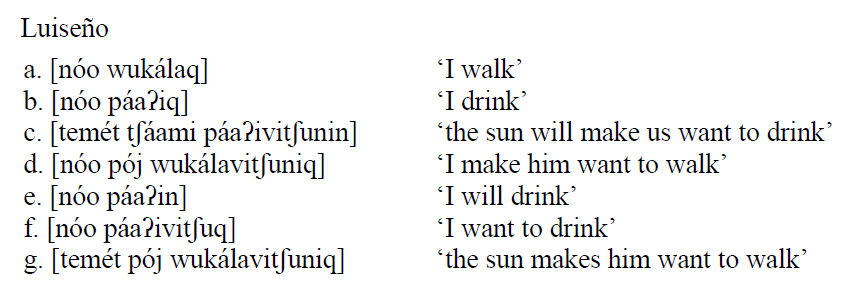
\includegraphics{../images/luiseno.png}
\end{figure}

~\\
INSTRUCTOR NOTES: ([temét])


~\\

{\large Question 22} (completed 20201001) - Source: Week 4 Handout, Part II, Question 3\\

Explain how you would figure out what the Luiseño form is for the morpheme whose meaning is given below. (To be clear: you do NOT need to give me the form itself -- just explain the process of figuring it out.)\\

‘drink’

\begin{figure}[H]
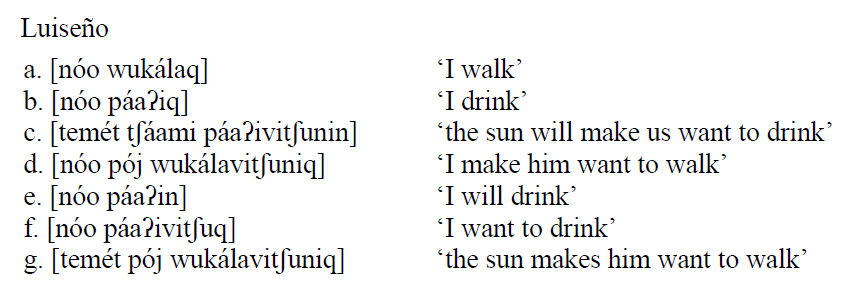
\includegraphics{../images/luiseno.png}
\end{figure}

~\\
INSTRUCTOR NOTES: ([páaʔi])


~\\

{\large Question 23} (completed 20201001) - Source: Week 4 Handout, Part II, Question 3\\

Explain how you would figure out what the Luiseño form is for the morpheme whose meaning is given below. (To be clear: you do NOT need to give me the form itself -- just explain the process of figuring it out.)\\

‘make / cause’

\begin{figure}[H]
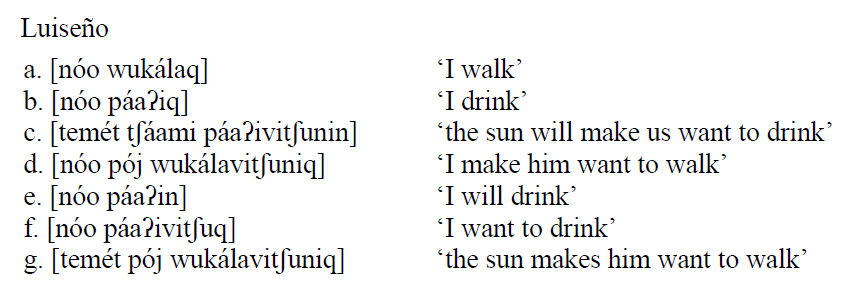
\includegraphics{../images/luiseno.png}
\end{figure}

~\\
INSTRUCTOR NOTES: ([ni])


~\\

{\large Question 24} (completed 20201001) - Source: Week 4 Handout, Part II, Question 3\\

Explain how you would figure out what the Luiseño form is for the morpheme whose meaning is given below. (To be clear: you do NOT need to give me the form itself -- just explain the process of figuring it out.)\\

‘Future’

\begin{figure}[H]
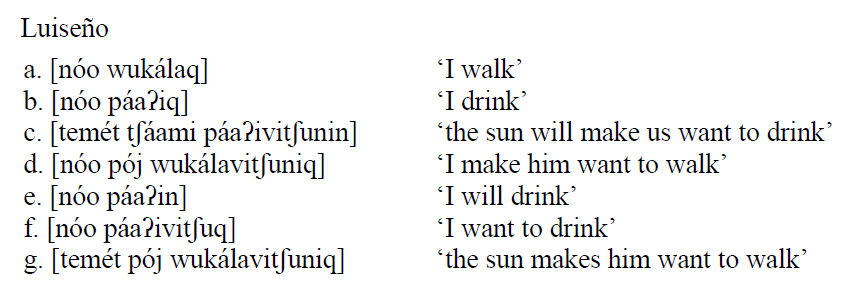
\includegraphics{../images/luiseno.png}
\end{figure}

~\\
INSTRUCTOR NOTES: ([n])


~\\

{\large Question 25} (completed 20201001) - Source: Week 4 Handout, Part II, Question 4\\

Explain how you could do morphological analysis on a signed language.\\


~\\
INSTRUCTOR NOTES: 


~\\

{\large Question 26} (completed 20201006) - Source: Week 5 Handout, Question 0\\

Explain what we mean by saying that linguistic patterns are \underline{productive}.\\


~\\
INSTRUCTOR NOTES: 


~\\

{\large Question 27} (completed -nodate-) - Source: \\

What would this Klingon phrase below be in English? How do you know?\\

{[pɑdɑq]}

\begin{figure}[H]
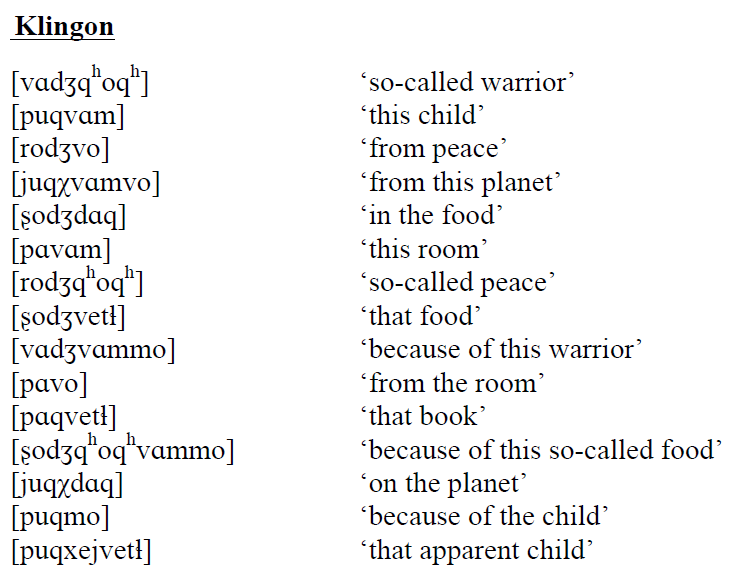
\includegraphics{../images/klingon.png}
\end{figure}

~\\
INSTRUCTOR NOTES: ‘in/on (the) room’


~\\

{\large Question 28} (completed -nodate-) - Source: \\

What would this Klingon phrase below be in English? How do you know?\\

{[vɑdʒqʰoqʰvɑm]}

\begin{figure}[H]
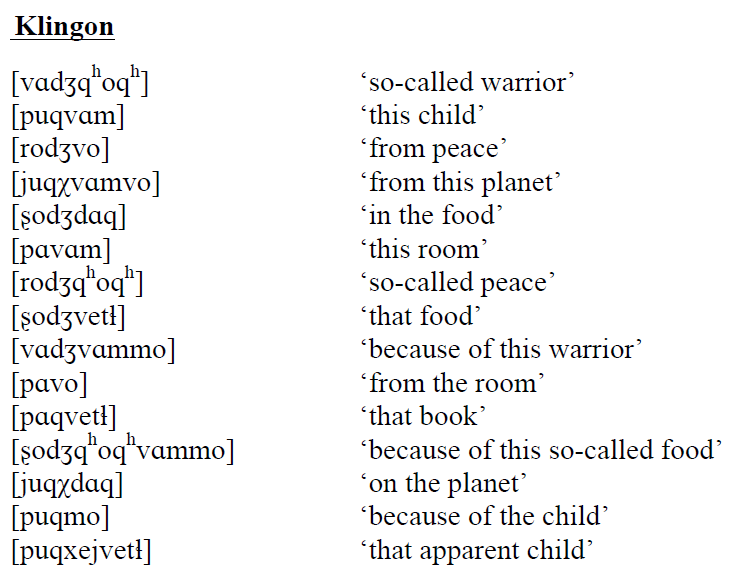
\includegraphics{../images/klingon.png}
\end{figure}

~\\
INSTRUCTOR NOTES: ‘this so-called warrior’


~\\

{\large Question 29} (completed -nodate-) - Source: \\

What would this Klingon phrase below be in English? How do you know?\\

{[pɑqqʰoqʰvetɬvo]}

\begin{figure}[H]
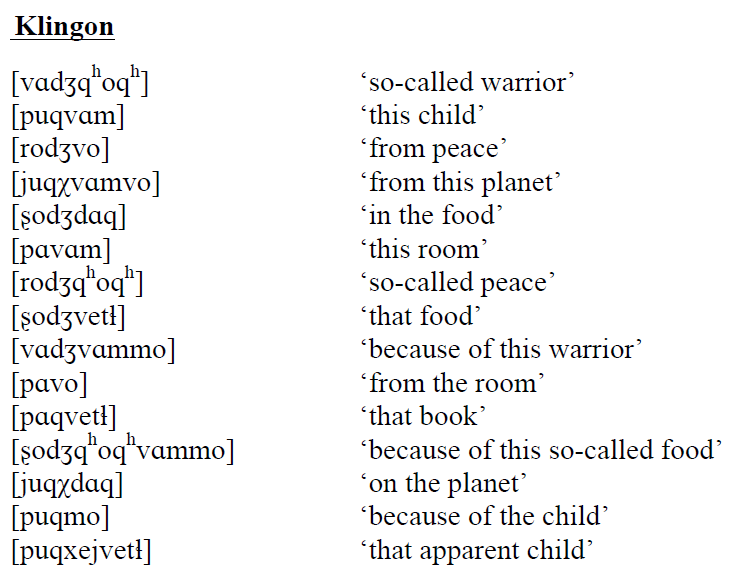
\includegraphics{../images/klingon.png}
\end{figure}

~\\
INSTRUCTOR NOTES: ‘from that so-called book’


\newpage\textbf{\underline{\huge Articulatory Phonetics / hard\\}}

~\\

{\large Question 1} (completed 20200918) - Source: Week 2 Discussion\\

Explain why it's possible to say that signed languages have articulatory phonetics.\\


~\\
INSTRUCTOR NOTES: 


~\\

{\large Question 2} (completed 20200925) - Source: Week 3 Handout, Question 3\\

Explain why the additional vowel below either does or does not belong in the phonetic natural class defined by the original set of SNAE vowels.\\

Original set: {[æ]}, {[ɑ]}

Addition: {[ɑʊ]}


~\\
INSTRUCTOR NOTES: should recognize that there's more than one vowel sound, which makes it somewhat difficult to categorize; best answers will say that the diphthong is crucially a diphthong and so can't also go in this class


~\\

{\large Question 3} (completed 20200925) - Source: Week 3 Handout, Question 3\\

Explain why the additional vowel below either does or does not belong in the phonetic natural class defined by the original set of SNAE vowels.\\

Original set: {[u]}, {[ʊ]}, {[oʊ]}, {[ɔ]}

Addition: {[ɔɪ]}


~\\
INSTRUCTOR NOTES: should recognize that there's more than one vowel sound, which makes it somewhat difficult to categorize; best answers will say that the diphthong is crucially a diphthong and so can't also go in this class


~\\

{\large Question 4} (completed 20200925) - Source: Week 3 Handout, Question 3\\

Explain why the additional vowel below either does or does not belong in the phonetic natural class defined by the original set of SNAE vowels.\\

Original set: {[ɛ]}, {[ɪ]}, {[ʊ]}, {[ɔ]}

Addition: {[æ]}


~\\
INSTRUCTOR NOTES: new vowel is a low vowel; should recognize that there's more than one decision about low vowels and tenseness; default is to say it doesn't belong in the class because tenseness is irrelevant


~\\

{\large Question 5} (completed 20200925) - Source: Week 3 Handout, Question 3\\

Explain why the additional vowel below either does or does not belong in the phonetic natural class defined by the original set of SNAE vowels.\\

Original set: {[æ]}, {[ɑ]}

Addition: {[ɑɪ]}


~\\
INSTRUCTOR NOTES: should recognize that there's more than one vowel sound, which makes it somewhat difficult to categorize; best answers will say that the diphthong is crucially a diphthong and so can't also go in this class


~\\

{\large Question 6} (completed 20200925) - Source: Week 3 Handout, Question 3\\

Explain why the additional vowel below either does or does not belong in the phonetic natural class defined by the original set of SNAE vowels.\\

Original set: {[u]}, {[ʊ]}, {[oʊ]}, {[ɔ]}

Addition: {[ɑʊ]}


~\\
INSTRUCTOR NOTES: should recognize that there's more than one vowel sound, which makes it somewhat difficult to categorize; best answers will say that the diphthong is crucially a diphthong and so can't also go in this class


~\\

{\large Question 7} (completed 20200925) - Source: Week 3 Handout, Question 3\\

Explain why the additional vowel below either does or does not belong in the phonetic natural class defined by the original set of SNAE vowels.\\

Original set: {[ɛ]}, {[ɪ]}, {[ʊ]}, {[ɔ]}

Addition: {[ɑ]}


~\\
INSTRUCTOR NOTES: new vowel is a low vowel; should recognize that there's more than one decision about low vowels and tenseness; default is to say it doesn't belong in the class because tenseness is irrelevant


~\\

{\large Question 8} (completed 20201001) - Source: Homework 1, Question 3(a)\\

Could this image be the result of producing the sound represented by the given IPA symbol? Why or why not?\\

{[d]}

\begin{figure}[H]
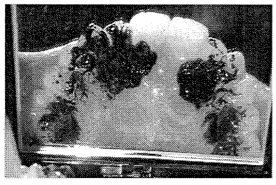
\includegraphics{../images/staticpalatography_fricative.png}
\end{figure}

~\\
INSTRUCTOR NOTES: no; space


~\\

{\large Question 9} (completed 20201001) - Source: Homework 1, Question 3(a)\\

Could this image be the result of producing the sound represented by the given IPA symbol? Why or why not?\\

{[z]}

\begin{figure}[H]
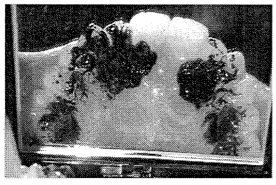
\includegraphics{../images/staticpalatography_fricative.png}
\end{figure}

~\\
INSTRUCTOR NOTES: yes


~\\

{\large Question 10} (completed 20201001) - Source: Homework 1, Question 3(a)\\

Could this image be the result of producing the sound represented by the given IPA symbol? Why or why not?\\

{[n]}

\begin{figure}[H]
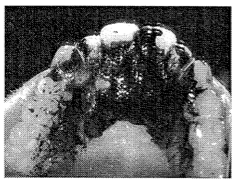
\includegraphics{../images/staticpalatography_stop.png}
\end{figure}

~\\
INSTRUCTOR NOTES: yes


~\\

{\large Question 11} (completed 20201001) - Source: Homework 1, Question 3(a)\\

Could this image be the result of producing the sound represented by the given IPA symbol? Why or why not?\\

{[t͡ʃ]}

\begin{figure}[H]
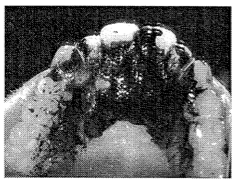
\includegraphics{../images/staticpalatography_stop.png}
\end{figure}

~\\
INSTRUCTOR NOTES: yes


~\\

{\large Question 12} (completed 20201001) - Source: Homework 1, Question 3(a)\\

Could this image be the result of producing the sound represented by the given IPA symbol? Why or why not?\\

{[t͡ʃ]}

\begin{figure}[H]
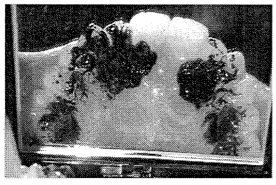
\includegraphics{../images/staticpalatography_fricative.png}
\end{figure}

~\\
INSTRUCTOR NOTES: no


~\\

{\large Question 13} (completed 20201001) - Source: Homework 1, Question 3(a)\\

Could this image be the result of producing the sound represented by the given IPA symbol? Why or why not?\\

{[ɾ]}

\begin{figure}[H]
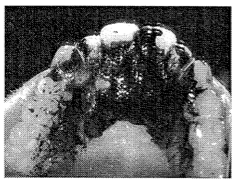
\includegraphics{../images/staticpalatography_stop.png}
\end{figure}

~\\
INSTRUCTOR NOTES: yes


\newpage\textbf{\underline{\huge Articulatory Phonetics / easy\\}}

~\\

{\large Question 1} (completed 20200915) - Source: Quiz 1, Question 12\\

Explain what this diagram tells you about the articulation of sounds.\\

\begin{figure}[H]
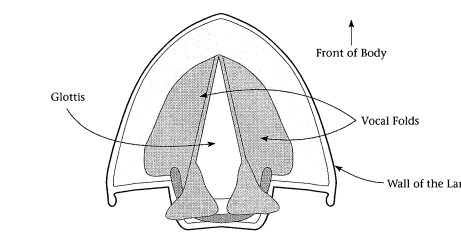
\includegraphics{../images/spreadglottis_diagram.png}
\end{figure}

~\\
INSTRUCTOR NOTES: 


~\\

{\large Question 2} (completed 20200918) - Source: Week 2 Handout, Part I, Question 12\\

Explain in what sense the difference between the sounds in the words <but> and <cut> is SIMILAR to and also DIFFERENT from the difference between the sounds in the words <bit> and <kit>.\\


~\\
INSTRUCTOR NOTES: 


~\\

{\large Question 3} (completed 20200925) - Source: Week 3 Discussion\\

Describe what the tongue would do / where it would move during each of the vowels in this word.\\

<vacuum>


~\\
INSTRUCTOR NOTES: 


~\\

{\large Question 4} (completed 20200925) - Source: Week 3 Discussion\\

Describe what the tongue would do / where it would move during each of the vowels in this word.\\

<puny>


~\\
INSTRUCTOR NOTES: 


~\\

{\large Question 5} (completed 20200925) - Source: Week 3 Discussion\\

Describe what the tongue would do / where it would move during each of the vowels in this word.\\

<follow>


~\\
INSTRUCTOR NOTES: 


~\\

{\large Question 6} (completed 20200925) - Source: Week 3 Handout, Question 7\\

Is the symbol given a reasonable way to transcribe any of the sounds described below? If so, which one? If not, why not?\\

{[n]}

\begin{itemize} \item voiceless palatal affricate \item voiced velar nasal \item voiceless glottal fricative \item voiced labiodental fricative \item voiced interdental fricative \item voiced palatal fricative \end{itemize}


~\\
INSTRUCTOR NOTES: no (voiced alveolar nasal)


~\\

{\large Question 7} (completed 20200925) - Source: Week 3 Handout, Question 7\\

Is the symbol given a reasonable way to transcribe any of the sounds described below? If so, which one? If not, why not?\\

{[h]}

\begin{itemize} \item voiceless palatal affricate \item voiced velar nasal \item voiceless glottal fricative \item voiced labiodental fricative \item voiced interdental fricative \item voiced palatal fricative \end{itemize}


~\\
INSTRUCTOR NOTES: yes (voiceless glottal fricative)


~\\

{\large Question 8} (completed 20200925) - Source: Week 3 Handout, Question 7\\

Is the symbol given a reasonable way to transcribe any of the sounds described below? If so, which one? If not, why not?\\

{[v]}

\begin{itemize} \item voiceless palatal affricate \item voiced velar nasal \item voiceless glottal fricative \item voiced labiodental fricative \item voiced interdental fricative \item voiced palatal fricative \end{itemize}


~\\
INSTRUCTOR NOTES: yes (voiced labiodental fricative)


~\\

{\large Question 9} (completed 20200925) - Source: Week 3 Handout, Question 7\\

Is the symbol given a reasonable way to transcribe any of the sounds described below? If so, which one? If not, why not?\\

{[θ]}

\begin{itemize} \item voiceless palatal affricate \item voiced velar nasal \item voiceless glottal fricative \item voiced labiodental fricative \item voiced interdental fricative \item voiced palatal fricative \end{itemize}


~\\
INSTRUCTOR NOTES: no (voiceless interdental fricative)


~\\

{\large Question 10} (completed 20200925) - Source: Week 3 Handout, Question 7\\

Is the symbol given a reasonable way to transcribe any of the sounds described below? If so, which one? If not, why not?\\

{[ʃ]}

\begin{itemize} \item voiceless palatal affricate \item voiced velar nasal \item voiceless glottal fricative \item voiced labiodental fricative \item voiced interdental fricative \item voiced palatal fricative \end{itemize}


~\\
INSTRUCTOR NOTES: no (voiceless palatal fricative)


~\\

{\large Question 11} (completed 20200925) - Source: Week 3 Handout, Question 7\\

Is the symbol given a reasonable way to transcribe any of the sounds described below? If so, which one? If not, why not?\\

{[ʒ]}

\begin{itemize} \item voiceless palatal affricate \item voiced velar nasal \item voiceless glottal fricative \item voiced labiodental fricative \item voiced interdental fricative \item voiced palatal fricative \end{itemize}


~\\
INSTRUCTOR NOTES: yes (voiced palatal fricative)


~\\

{\large Question 12} (completed 20200925) - Source: Week 3 Handout, Question 7\\

Is the symbol given a reasonable way to transcribe any of the sounds described below? If so, which one? If not, why not?\\

{[t͡ʃ]}

\begin{itemize} \item voiceless palatal affricate \item voiced velar nasal \item voiceless glottal fricative \item voiced labiodental fricative \item voiced interdental fricative \item voiced palatal fricative \end{itemize}


~\\
INSTRUCTOR NOTES: yes (voiceless palatal affricate)


\newpage\textbf{\underline{\huge Articulatory Phonetics / medium\\}}

~\\

{\large Question 1} (completed 20200925) - Source: Week 3 Discussion\\

Assuming a Standard North American English inventory, does this vowel need to have tenseness specified if you're giving a prose description? Why or why not?\\

{[æ]}


~\\
INSTRUCTOR NOTES: no


~\\

{\large Question 2} (completed 20200925) - Source: Week 3 Discussion\\

Assuming a Standard North American English inventory, does this vowel need to have tenseness specified if you're giving a prose description? Why or why not?\\

{[ɑ]}


~\\
INSTRUCTOR NOTES: no


~\\

{\large Question 3} (completed 20200925) - Source: Week 3 Discussion\\

Assuming a Standard North American English inventory, does this vowel need to have tenseness specified if you're giving a prose description? Why or why not?\\

{[i]}


~\\
INSTRUCTOR NOTES: yes


~\\

{\large Question 4} (completed 20200925) - Source: Week 3 Discussion\\

Assuming a Standard North American English inventory, does this vowel need to have tenseness specified if you're giving a prose description? Why or why not?\\

{[u]}


~\\
INSTRUCTOR NOTES: yes


~\\

{\large Question 5} (completed 20200925) - Source: Week 3 Discussion\\

Assuming a Standard North American English inventory, does this vowel need to have tenseness specified if you're giving a prose description? Why or why not?\\

{[ɛ]}


~\\
INSTRUCTOR NOTES: yes


~\\

{\large Question 6} (completed 20200925) - Source: Week 3 Discussion\\

Assuming a Standard North American English inventory, does this vowel need to have tenseness specified if you're giving a prose description? Why or why not?\\

{[ɔ]}


~\\
INSTRUCTOR NOTES: yes


~\\

{\large Question 7} (completed 20200925) - Source: Week 3 Discussion\\

Describe what the tongue would do / where it would move during each of the vowels in this word.\\

<bookmark>


~\\
INSTRUCTOR NOTES: 


~\\

{\large Question 8} (completed 20200925) - Source: Week 3 Discussion\\

Describe what the tongue would do / where it would move during each of the vowels in this word.\\

<waitlist>


~\\
INSTRUCTOR NOTES: 


~\\

{\large Question 9} (completed 20200925) - Source: Week 3 Discussion\\

Describe what the tongue would do / where it would move during each of the vowels in this word.\\

<July>


~\\
INSTRUCTOR NOTES: 


~\\

{\large Question 10} (completed 20200922) - Source: Quiz 2, Question 6\\

In the pronunciation of this word, which sounds are obstruents and which are sonorants?\\

<sonorant>


~\\
INSTRUCTOR NOTES: [sɔnoɹənt] -- sonorants: [ɔnoɹən] and obstruents: [st]


~\\

{\large Question 11} (completed 20200922) - Source: Quiz 2, Question 6\\

In the pronunciation of this word, which sounds are obstruents and which are sonorants?\\

<obstruent>


~\\
INSTRUCTOR NOTES: [ɑbstɹuənt] -- sonorants: [ɑɹuən] and obstruents: [bstt]


~\\

{\large Question 12} (completed 20200922) - Source: Quiz 2, Question 6\\

In the pronunciation of this word, which sounds are obstruents and which are sonorants?\\

<language>


~\\
INSTRUCTOR NOTES: [læŋɡwɪdʒ] -- sonorants: [læŋwɪ] and obstruents: [ɡdʒ]


~\\

{\large Question 13} (completed 20200922) - Source: Quiz 2, Question 6\\

In the pronunciation of this word, which sounds are obstruents and which are sonorants?\\

<fricative>


~\\
INSTRUCTOR NOTES: [fɹɪkətɪv] -- sonorants: [ɹɪəɪ] and obstruents: [fktv]


~\\

{\large Question 14} (completed 20200922) - Source: Quiz 2, Question 7\\

Why might more than one of the descriptions given truthfully apply to the sound represented by the underlined letter, and why is one of them actually better than the other?\\

<a\underline{w}ay>

\begin{itemize} \item prevocalic obstruent \item prevocalic sonorant \item postvocalic obstruent \item postvocalic sonorant \item intervocalic obstruent \item intervocalic sonorant \end{itemize}


~\\
INSTRUCTOR NOTES: prevocalic and *intervocalic* sonorant


~\\

{\large Question 15} (completed 20200925) - Source: Week 3 Handout, Question 9\\

Explain how to figure out what the sound being produced is in this diagram.\\

\begin{figure}[H]
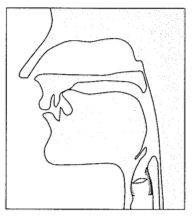
\includegraphics{../images/sagittal_t.png}
\end{figure}

~\\
INSTRUCTOR NOTES: [t] (check voicing, place, manner, and velum)


~\\

{\large Question 16} (completed 20200925) - Source: Week 3 Handout, Question 9\\

Explain how to figure out what the sound being produced is in this diagram.\\

\begin{figure}[H]
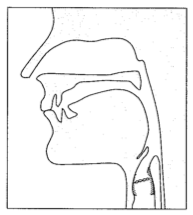
\includegraphics{../images/sagittal_m.png}
\end{figure}

~\\
INSTRUCTOR NOTES: [m] (check voicing, place, manner, and velum)


~\\

{\large Question 17} (completed 20200925) - Source: Week 3 Handout, Question 9\\

Explain how to figure out what the sound being produced is in this diagram.\\

\begin{figure}[H]
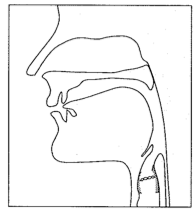
\includegraphics{../images/sagittal_eth.png}
\end{figure}

~\\
INSTRUCTOR NOTES: [ð] (check voicing, place, manner, and velum)


~\\

{\large Question 18} (completed 20200925) - Source: Week 3 Handout, Question 9\\

Explain how to figure out what the sound being produced is in this diagram.\\

\begin{figure}[H]
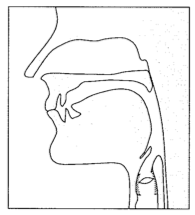
\includegraphics{../images/sagittal_p.png}
\end{figure}

~\\
INSTRUCTOR NOTES: [p] (check voicing, place, manner, and velum)


~\\

{\large Question 19} (completed 20200925) - Source: Week 3 Handout, Question 9\\

Explain how to figure out what the sound being produced is in this diagram.\\

\begin{figure}[H]
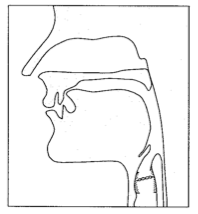
\includegraphics{../images/sagittal_z.png}
\end{figure}

~\\
INSTRUCTOR NOTES: [z] (check voicing, place, manner, and velum)


~\\

{\large Question 20} (completed 20200925) - Source: Week 3 Handout, Question 13\\

Explain why this image does or does not match the description.\\

\begin{itemize} \item A two-handed sign. \item Location: In front of signer’s chin. \item Handshape: Starts with an “L” shape; index finger and thumb come together during the sign. \item Movement: Hands start crossed and then move away from each other horizontally. \end{itemize}

\begin{figure}[H]
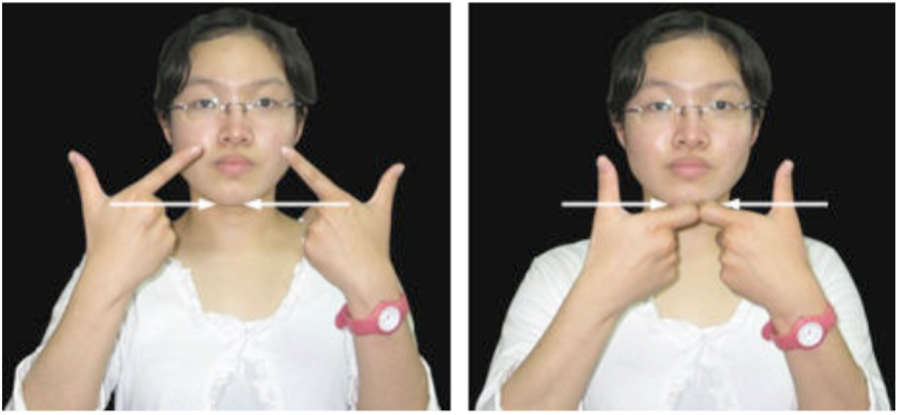
\includegraphics{../images/taiwansign_fit.png}
\caption{FIT}
\end{figure}

~\\
INSTRUCTOR NOTES: no; hands don't start crossed, and handshape change is wrong


~\\

{\large Question 21} (completed 20200925) - Source: Week 3 Handout, Question 13\\

Explain why this image does or does not match the description.\\

\begin{itemize} \item A two-handed sign. \item Location: In front of signer’s chin. \item Handshape: Starts with an “L” shape; distal joints of index fingers fold in during the sign. \item Movement: Hands start apart and then move straight toward each other horizontally. \end{itemize}

\begin{figure}[H]
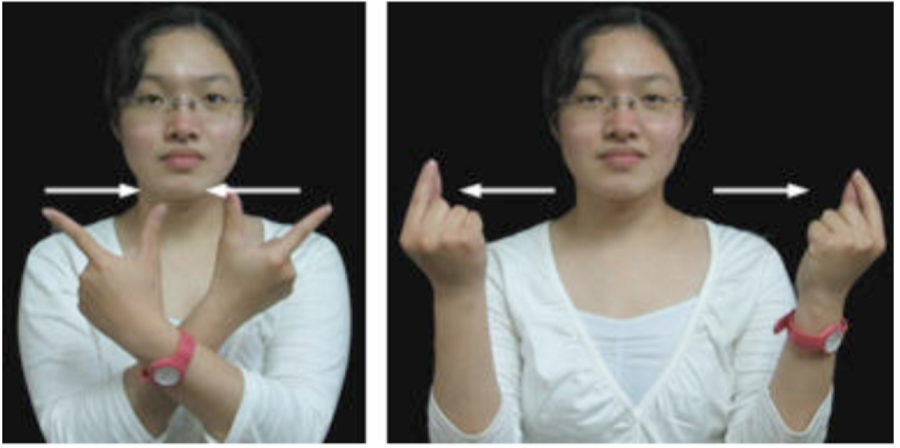
\includegraphics{../images/taiwansign_consistent.png}
\caption{CONSISTENT}
\end{figure}

~\\
INSTRUCTOR NOTES: no; hands don't start apart, and handshape change is wrong


~\\

{\large Question 22} (completed 20200925) - Source: Week 3 Handout, Question 13\\

Explain why this image does or does not match the description.\\

\begin{itemize} \item A one-handed sign. \item Location: At the signer’s nose. \item Handshape: Starts with index finger extended; finger folds down into a “hook” shape during the sign; then straightens and repeats the folding. \item Movement: No movement other than the change in handshape. \end{itemize}

\begin{figure}[H]
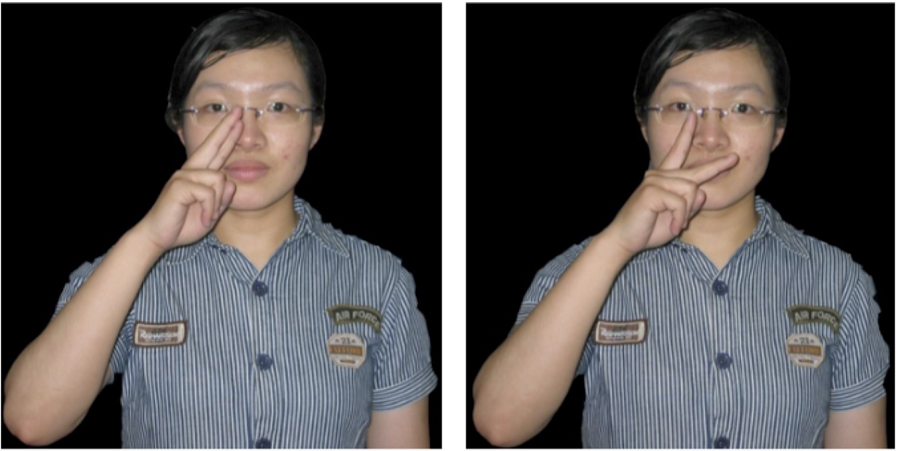
\includegraphics{../images/taiwansign_wrong.png}
\caption{WRONG}
\end{figure}

~\\
INSTRUCTOR NOTES: no; handshape is wrong


~\\

{\large Question 23} (completed 20200925) - Source: Week 3 Handout, Question 13\\

Explain why this image does or does not match the description.\\

\begin{itemize} \item A one-handed sign. \item Location: In front of signer’s chin. \item Handshape: Starts with an “L” shape; proximal joint of index finger folds down during the sign. \item Movement: Hand starts on far side of signer’s body and moves horizontally straight across. \end{itemize}

\begin{figure}[H]
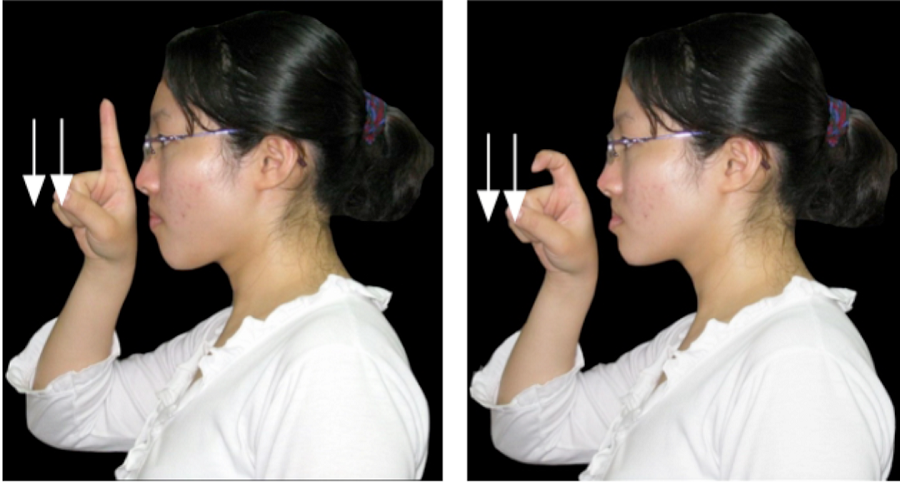
\includegraphics{../images/taiwansign_jealous.png}
\caption{JEALOUS}
\end{figure}

~\\
INSTRUCTOR NOTES: no; handshape and movement are wrong


~\\

{\large Question 24} (completed 20200925) - Source: Week 3 Handout, Question 13\\

Explain why this image does or does not match the description.\\

\begin{itemize} \item A one-handed sign. \item Location: At the signer’s nose. \item Handshape: Starts with index and middle finger crossed; the two fingers separate during the sign. \item Movement: No movement other than the change in handshape. \end{itemize}

\begin{figure}[H]
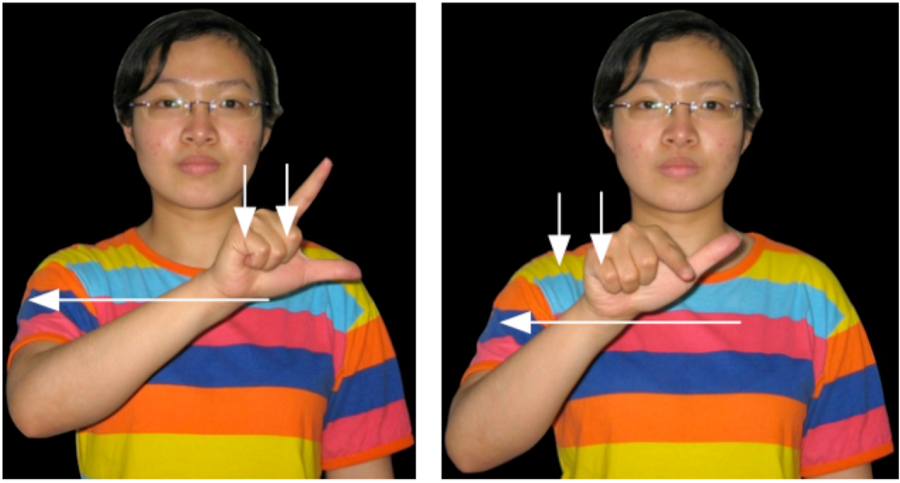
\includegraphics{../images/taiwansign_thing.png}
\caption{THING}
\end{figure}

~\\
INSTRUCTOR NOTES: no; location, movement, and handshape are all wrong


~\\

{\large Question 25} (completed 20201001) - Source: Homework 1, Question 3(b)\\

Explain why this is or is not a complete phonetic natural class in standard North American English.\\

{[p]}, {[b]}


~\\
INSTRUCTOR NOTES: yes for bilabial plosives; (no) for bilabial stops (nasal?)


~\\

{\large Question 26} (completed 20201001) - Source: Homework 1, Question 3(b)\\

Explain why this is or is not a complete phonetic natural class in standard North American English.\\

{[f]}, {[s]}, {[ʃ]}


~\\
INSTRUCTOR NOTES: no; voiceless fricatives include [θ], [h]


~\\

{\large Question 27} (completed 20201001) - Source: Homework 1, Question 3(b)\\

Explain why this is or is not a complete phonetic natural class in standard North American English.\\

{[b]}, {[n]}, {[ɡ]}, {[ʒ]}, {[v]}


~\\
INSTRUCTOR NOTES: no; lots of other voiced consonants


~\\

{\large Question 28} (completed 20201001) - Source: Homework 1, Question 3(b)\\

Explain why this is or is not a complete phonetic natural class in standard North American English.\\

{[f]}, {[θ]}, {[z]}, {[h]}


~\\
INSTRUCTOR NOTES: no; several fricatives missing


~\\

{\large Question 29} (completed 20201001) - Source: Homework 1, Question 3(b)\\

Explain why this is or is not a complete phonetic natural class in standard North American English.\\

{[j]}, {[w]}


~\\
INSTRUCTOR NOTES: yes for voiced glides; [w̥] missing for glides


~\\

{\large Question 30} (completed 20201001) - Source: Homework 1, Question 3(b)\\

Explain why this is or is not a complete phonetic natural class in standard North American English.\\

{[ɑ]}, {[u]}


~\\
INSTRUCTOR NOTES: no; several back vowels / back monophthongs missing


~\\

{\large Question 31} (completed 20201001) - Source: Homework 1, Question 3(b)\\

Explain why this is or is not a complete phonetic natural class in standard North American English.\\

{[ɔ]}, {[ʊ]}, {[u]}, {[oʊ]}


~\\
INSTRUCTOR NOTES: yes (all back rounded vowels)


~\\

{\large Question 32} (completed 20201001) - Source: Homework 1, Question 3(b)\\

Explain why this is or is not a complete phonetic natural class in standard North American English.\\

{[i]}, {[u]}, {[eɪ]}


~\\
INSTRUCTOR NOTES: no; [oʊ] missing for tense vowels


\newpage\textbf{\underline{\huge Transcription / easy\\}}

~\\

{\large Question 1} (completed 20200915) - Source: Quiz 1, Question 10\\

Explain whether this word either does or does not have an [ʃ] sound in it, and why the spelling and pronunciation either do or do not align.\\

<shoe>


~\\
INSTRUCTOR NOTES: 


~\\

{\large Question 2} (completed 20200915) - Source: Quiz 1, Question 10\\

Explain whether this word either does or does not have an [ʃ] sound in it, and why the spelling and pronunciation either do or do not align.\\

<lotion>


~\\
INSTRUCTOR NOTES: 


~\\

{\large Question 3} (completed 20200915) - Source: Quiz 1, Question 10\\

Explain whether this word either does or does not have an [ʃ] sound in it, and why the spelling and pronunciation either do or do not align.\\

<facial>


~\\
INSTRUCTOR NOTES: 


~\\

{\large Question 4} (completed 20200915) - Source: Quiz 1, Question 10\\

Explain whether this word either does or does not have an [ʃ] sound in it, and why the spelling and pronunciation either do or do not align.\\

<sure>


~\\
INSTRUCTOR NOTES: 


~\\

{\large Question 5} (completed 20200915) - Source: Quiz 1, Question 10\\

Explain whether this word either does or does not have an [ʃ] sound in it, and why the spelling and pronunciation either do or do not align.\\

<passion>


~\\
INSTRUCTOR NOTES: 


~\\

{\large Question 6} (completed 20200915) - Source: Quiz 1, Question 10\\

Explain whether this word either does or does not have an [ʃ] sound in it, and why the spelling and pronunciation either do or do not align.\\

<mishandle>


~\\
INSTRUCTOR NOTES: 


~\\

{\large Question 7} (completed 20200915) - Source: Quiz 1, Question 10\\

Explain whether this word either does or does not have an [ʃ] sound in it, and why the spelling and pronunciation either do or do not align.\\

<super>


~\\
INSTRUCTOR NOTES: 


~\\

{\large Question 8} (completed 20200915) - Source: Quiz 1, Question 10\\

Explain whether this word either does or does not have an [ʃ] sound in it, and why the spelling and pronunciation either do or do not align.\\

<maniacal>


~\\
INSTRUCTOR NOTES: 


~\\

{\large Question 9} (completed 20200915) - Source: Quiz 1, Question 10\\

Explain whether this word either does or does not have an [ʃ] sound in it, and why the spelling and pronunciation either do or do not align.\\

<bassoon>


~\\
INSTRUCTOR NOTES: 


~\\

{\large Question 10} (completed 20200915) - Source: Quiz 1, Question 10\\

Explain whether this word either does or does not have an [ʃ] sound in it, and why the spelling and pronunciation either do or do not align.\\

<meticulous>


~\\
INSTRUCTOR NOTES: 


~\\

{\large Question 11} (completed 20200918) - Source: Week 2 Handout, Part II, Question 2\\

Explain why people might legitimately disagree about how many sounds this particular word contains.\\

<how>


~\\
INSTRUCTOR NOTES: 


~\\

{\large Question 12} (completed 20200918) - Source: Week 2 Handout, Part II, Question 2\\

Explain why people might legitimately disagree about how many sounds this particular word contains.\\

<tiny>


~\\
INSTRUCTOR NOTES: 


~\\

{\large Question 13} (completed 20200918) - Source: Week 2 Handout, Part II, Question 2\\

Explain why people might legitimately disagree about how many sounds this particular word contains.\\

<goat>


~\\
INSTRUCTOR NOTES: 


~\\

{\large Question 14} (completed 20200918) - Source: Week 2 Handout, Part II, Question 2\\

Explain why people might legitimately disagree about how many sounds this particular word contains.\\

<those>


~\\
INSTRUCTOR NOTES: 


~\\

{\large Question 15} (completed 20200918) - Source: Week 2 Handout, Part II, Question 2\\

Explain why people might legitimately disagree about how many sounds this particular word contains.\\

<flowers>


~\\
INSTRUCTOR NOTES: 


~\\

{\large Question 16} (completed 20200918) - Source: Week 2 Handout, Part II, Question 2\\

Explain why people might legitimately disagree about how many sounds this particular word contains.\\

<girls>


~\\
INSTRUCTOR NOTES: 


~\\

{\large Question 17} (completed 20200918) - Source: Week 2 Handout, Part II, Question 2\\

Explain why people might legitimately disagree about how many sounds this particular word contains.\\

<find>


~\\
INSTRUCTOR NOTES: 


~\\

{\large Question 18} (completed 20200918) - Source: Week 2 Handout, Part II, Question 2\\

Explain why people might legitimately disagree about how many sounds this particular word contains.\\

<they>


~\\
INSTRUCTOR NOTES: 


~\\

{\large Question 19} (completed 20200918) - Source: Week 2 Handout, Part II, Question 3\\

Explain why people might legitimately disagree about how many sounds this particular word contains.\\

<soap>


~\\
INSTRUCTOR NOTES: 


~\\

{\large Question 20} (completed 20200918) - Source: Week 2 Handout, Part II, Question 3\\

Explain why people might legitimately disagree about how many sounds this particular word contains.\\

<curtain>


~\\
INSTRUCTOR NOTES: 


~\\

{\large Question 21} (completed 20200918) - Source: Week 2 Handout, Part II, Question 3\\

Explain why people might legitimately disagree about how many sounds this particular word contains.\\

<better>


~\\
INSTRUCTOR NOTES: 


~\\

{\large Question 22} (completed 20200918) - Source: Week 2 Handout, Part II, Question 3\\

Explain why people might legitimately disagree about how many sounds this particular word contains.\\

<worse>


~\\
INSTRUCTOR NOTES: 


~\\

{\large Question 23} (completed 20200918) - Source: Week 2 Handout, Part II, Question 3\\

Explain why people might legitimately disagree about how many sounds this particular word contains.\\

<burger>


~\\
INSTRUCTOR NOTES: 


~\\

{\large Question 24} (completed 20200918) - Source: Week 2 Handout, Part II, Question 3\\

Explain why people might legitimately disagree about how many sounds this particular word contains.\\

<rice>


~\\
INSTRUCTOR NOTES: 


\newpage\textbf{\underline{\huge Transcription / medium\\}}

~\\

{\large Question 1} (completed 20200918) - Source: Week 2 Handout, Part II, Question 11\\

How would this word be transcribed?\\ Kathleen will likely ask a follow-up question about why you used a particular symbol.\\

<nice>


~\\
INSTRUCTOR NOTES: [nɑɪs]


~\\

{\large Question 2} (completed 20200918) - Source: Week 2 Handout, Part II, Question 11\\

How would this word be transcribed?\\ Kathleen will likely ask a follow-up question about why you used a particular symbol.\\

<frog>


~\\
INSTRUCTOR NOTES: [fɹɑɡ]


~\\

{\large Question 3} (completed 20200918) - Source: Week 2 Handout, Part II, Question 11\\

How would this word be transcribed?\\ Kathleen will likely ask a follow-up question about why you used a particular symbol.\\

<cough>


~\\
INSTRUCTOR NOTES: [kɑf]


~\\

{\large Question 4} (completed 20200918) - Source: Week 2 Handout, Part II, Question 11\\

How would this word be transcribed?\\ Kathleen will likely ask a follow-up question about why you used a particular symbol.\\

<juice>


~\\
INSTRUCTOR NOTES: [dʒus]


~\\

{\large Question 5} (completed 20200918) - Source: Week 2 Handout, Part II, Question 11\\

How would this word be transcribed?\\ Kathleen will likely ask a follow-up question about why you used a particular symbol.\\

<wealth>


~\\
INSTRUCTOR NOTES: [wɛlθ]


~\\

{\large Question 6} (completed 20200918) - Source: Week 2 Handout, Part II, Question 11\\

How would this word be transcribed?\\ Kathleen will likely ask a follow-up question about why you used a particular symbol.\\

<toy>


~\\
INSTRUCTOR NOTES: [tɔɪ]


~\\

{\large Question 7} (completed 20200918) - Source: Week 2 Handout, Part II, Question 11\\

How would this word be transcribed?\\ Kathleen will likely ask a follow-up question about why you used a particular symbol.\\

<finger>


~\\
INSTRUCTOR NOTES: [fɪŋɡɹ̩]


~\\

{\large Question 8} (completed 20200918) - Source: Week 2 Handout, Part II, Question 11\\

How would this word be transcribed?\\ Kathleen will likely ask a follow-up question about why you used a particular symbol.\\

<little>


~\\
INSTRUCTOR NOTES: [lɪɾl̩]


~\\

{\large Question 9} (completed 20200918) - Source: Week 2 Handout, Part II, Question 11\\

How would this word be transcribed?\\ Kathleen will likely ask a follow-up question about why you used a particular symbol.\\

<vacuum>


~\\
INSTRUCTOR NOTES: [vækjum]


~\\

{\large Question 10} (completed 20200918) - Source: Week 2 Handout, Part II, Question 11\\

How would this word be transcribed?\\ Kathleen will likely ask a follow-up question about why you used a particular symbol.\\

<bird>


~\\
INSTRUCTOR NOTES: [bɹ̩d]


~\\

{\large Question 11} (completed 20200918) - Source: Week 2 Handout, Part II, Question 11\\

How would this word be transcribed?\\ Kathleen will likely ask a follow-up question about why you used a particular symbol.\\

<segment>


~\\
INSTRUCTOR NOTES: [sɛɡmɛnt]


~\\

{\large Question 12} (completed 20200918) - Source: Week 2 Handout, Part II, Question 11\\

How would this word be transcribed?\\ Kathleen will likely ask a follow-up question about why you used a particular symbol.\\

<square>


~\\
INSTRUCTOR NOTES: [skweɪɹ]


~\\

{\large Question 13} (completed 20200918) - Source: Week 2 Handout, Part II, Question 11\\

How would this word be transcribed?\\ Kathleen will likely ask a follow-up question about why you used a particular symbol.\\

<goat>


~\\
INSTRUCTOR NOTES: [ɡoʊt]


\newpage\textbf{\underline{\huge Transcription / hard\\}}

~\\

{\large Question 1} (completed 20200918) - Source: Week 2 Handout, Part II\\

Is this a reasonable transcription of this word? Explain why.\\

<mouse>: {[mɔɪs]}


~\\
INSTRUCTOR NOTES: no, [ɑʊ]


~\\

{\large Question 2} (completed 20200918) - Source: Week 2 Handout, Part II\\

Is this a reasonable transcription of this word? Explain why.\\

<loud>: {[lɑud]}


~\\
INSTRUCTOR NOTES: okay, but [ɑʊ]


~\\

{\large Question 3} (completed 20200918) - Source: Week 2 Handout, Part II\\

Is this a reasonable transcription of this word? Explain why.\\

<philosophy>: {[fəlɑsəfi]}


~\\
INSTRUCTOR NOTES: yes


~\\

{\large Question 4} (completed 20200918) - Source: Week 2 Handout, Part II\\

Is this a reasonable transcription of this word? Explain why.\\

<choose>: {[t͡ʃuz]}


~\\
INSTRUCTOR NOTES: yes


~\\

{\large Question 5} (completed 20200918) - Source: Week 2 Handout, Part II\\

Is this a reasonable transcription of this word? Explain why.\\

<wimp>: {[wimp]}


~\\
INSTRUCTOR NOTES: no, [ɪ]


~\\

{\large Question 6} (completed 20200918) - Source: Week 2 Handout, Part II\\

Is this a reasonable transcription of this word? Explain why.\\

<paid>: {[peid]}


~\\
INSTRUCTOR NOTES: okay, but [eɪ]


~\\

{\large Question 7} (completed 20200918) - Source: Week 2 Handout, Part II\\

Is this a reasonable transcription of this word? Explain why.\\

<climb>: {[klɑɪm]}


~\\
INSTRUCTOR NOTES: yes


~\\

{\large Question 8} (completed 20200918) - Source: Week 2 Handout, Part II\\

Is this a reasonable transcription of this word? Explain why.\\

<shows>: {[ʃoʊs]}


~\\
INSTRUCTOR NOTES: no, [z]


~\\

{\large Question 9} (completed 20200918) - Source: Week 2 Handout, Part II\\

Is this a reasonable transcription of this word? Explain why.\\

<mine>: {[mɑɪn]}


~\\
INSTRUCTOR NOTES: yes


~\\

{\large Question 10} (completed 20200918) - Source: Week 2 Handout, Part II\\

Is this a reasonable transcription of this word? Explain why.\\

<health>: {[hɛlð]}


~\\
INSTRUCTOR NOTES: no, [θ]


\newpage\textbf{\underline{\huge Skewed Distributions / medium\\}}

~\\

{\large Question 1} (completed 20201006) - Source: Quiz 4, Question 1\\

L$_X$ (Language X) has three vowels, [i], [a], and [u]. It has bi-syllabic roots like Kikuyu. It does not allow non-identical high vowels to co-occur. Of the following nine logically possible vocalic sequences, which ones should be unattested in L$_X$? Explain why.\\

\begin{itemize} \item {[i...i]} \item {[i...a]} \item {[i...u]} \item {[a...i]} \item {[a...a]} \item {[a...u]} \item {[u...i]} \item {[u...a]} \item {[u...u]} \end{itemize}


~\\
INSTRUCTOR NOTES: [i...u], [u...i]


~\\

{\large Question 2} (completed 20201006) - Source: Quiz 4, Question 2\\

L$_X$ (Language X) has three vowels, [i], [a], and [u]. L$_X$ has tri-syllabic roots. If L$_X$ does not allow non-identical high vowels to co-occur, which one of the following tri-syllabic vocalic sequences do you predict to be unattested in L$_X$? Explain why.\\

\begin{itemize} \item {[u...i...a]} \item {[a...i...a]} \item {[u...u...a]} \item {[a...i...i]} \end{itemize}


~\\
INSTRUCTOR NOTES: [u...i...a]


~\\

{\large Question 3} (completed 20201006) - Source: Week 5 Handout, Question 1\\

Explain why we think that languages are not random in terms of their phonology.\\


~\\
INSTRUCTOR NOTES: 


~\\

{\large Question 4} (completed 20201006) - Source: Week 5 Handout, Question 3\\

What evidence is there that there is a pattern in these data, assuming that these are the only CV and VC sequences that occur in some language?\\

{[sa]}, {[ʃi]}, {[za]}, {[ʒi]}, {[as]}, {[iʃ]}, {[az]}, {[iʒ]}


~\\
INSTRUCTOR NOTES: (the palatal sounds occur with the high vowel, while the alveolar sounds occur with the low vowel)


~\\

{\large Question 5} (completed 20201008) - Source: Week 5 Handout, Question 5\\

How would you look for co-occurrence restrictions between [s] and the vowels that come after it in this dataset?\\

\begin{figure}[H]
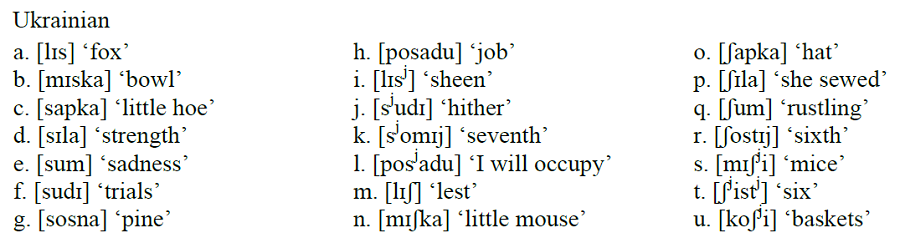
\includegraphics{../images/ukrainian.png}
\end{figure}

~\\
INSTRUCTOR NOTES: 


~\\

{\large Question 6} (completed 20201006) - Source: Week 5 Handout, Question 4\\

Explain why it's not reasonable to make any of the following claims about Phonologese.\\

\begin{figure}[H]
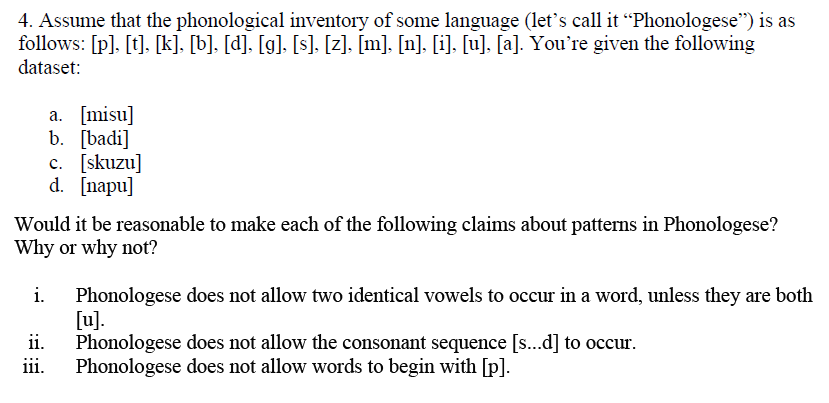
\includegraphics{../images/Phonologese.png}
\end{figure}

~\\
INSTRUCTOR NOTES: Not enough data to make any of these claims.


\newpage\textbf{\underline{\huge Skewed Distributions / easy\\}}

~\\

{\large Question 1} (completed 20201006) - Source: Week 5 Handout, Question 2\\

Explain why there should only be 8 sequences listed in the answer, even though multiplying 4 x 4 would give you 16 possible sequences.\\


~\\
INSTRUCTOR NOTES: The instructions say that you're only supposed to consider CV and VC sequences. 


~\\

{\large Question 2} (completed 20201008) - Source: Week 5 Handout, Question 6\\

Explain why the following table would not be a good way of organizing the data for Malto.\\

\begin{figure}[H]
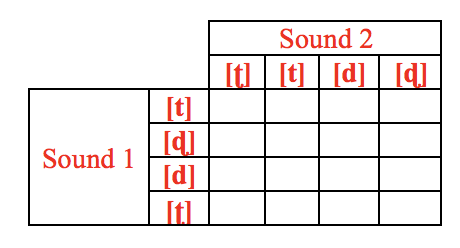
\includegraphics{../images/Malto_table_bad.png}
\end{figure}

~\\
INSTRUCTOR NOTES: rows and columns not in same order; rows not organized by phonetic characteristic; specifically, instructions ask about dental vs. retroflex, so should be organized around those


~\\

{\large Question 3} (completed 20201008) - Source: Week 5 Handout, Question 5\\

Explain why it is possible to predict which of [s] or [ʃʲ] will occur in a new environment in Ukrainian, but not possible to predict which of [s] or [ʃ] will occur in a new environment.\\


~\\
INSTRUCTOR NOTES: [s] and [S] have the same pattern of co-occurrence restrictions, so they occur in the same environments, and you cannot predict which one will occur where. [s] and [Sj] on the other hand have 'opposite' patterns, so you can always predict which will occur based on the vowel.


\newpage\textbf{\underline{\huge Skewed Distributions / hard\\}}

~\\

{\large Question 1} (completed 20201008) - Source: Week 5 Handout, Question 7\\

Explain how you would go about looking for co-occurrence restrictions in bi-syllabic signs in ASL.\\

\begin{figure}[H]
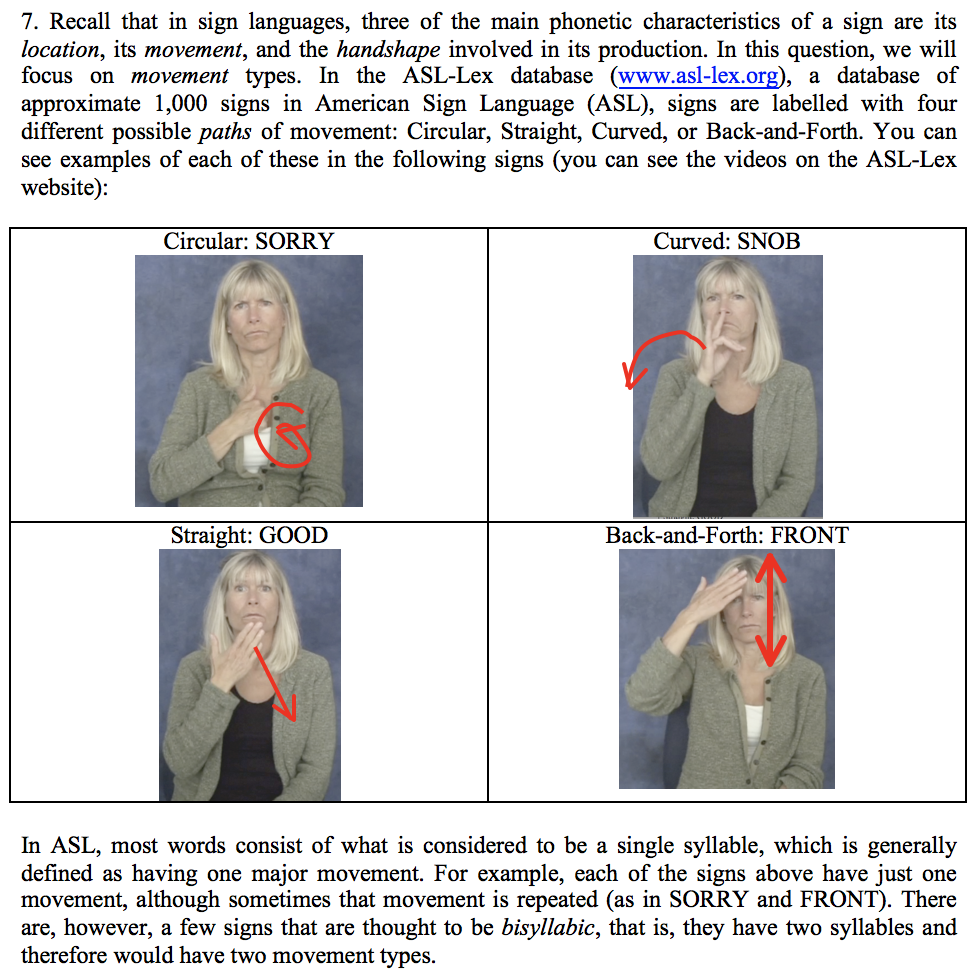
\includegraphics{../images/ASL_movement.png}
\end{figure}

~\\
INSTRUCTOR NOTES: You would start by coming up with all the possible combinations expected (i.e., 4x4 = 16). Then you'd compare that to some database of signs in ASL and see which combinations are actually attested or unattested.


~\\

{\large Question 2} (completed 20201008) - Source: Week 5 Handout, Question 5\\

Explain why looking for patterns with consonants and vowels is a more reasonable approach to pattern finding in this dataset than looking for patterns with respect to all of the individual sounds in Ukrainian.\\

\begin{figure}[H]
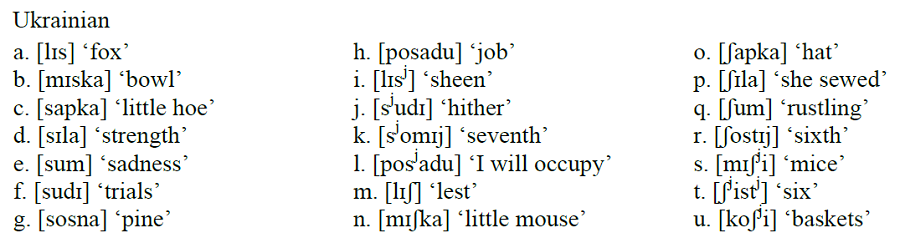
\includegraphics{../images/ukrainian.png}
\end{figure}

~\\
INSTRUCTOR NOTES: Collapsing sounds into "consonants" and "vowels" allows us to have 'sufficient data' in a way that thinking about all the individual combinations of sounds would not.


~\\

{\large Question 3} (completed 20201008) - Source: Week 5 Handout, Question 6\\

If I gave you a new word in Malto, [di\_\_u], would it be possible to predict whether it's [d] or [ɖ] that goes in the blank? Explain why or why not.\\


~\\
INSTRUCTOR NOTES: Yes, it's possible; in Malto, if there are two stops in a word, they must either both be dental or both retroflex. Since the first sound is dental, the second must also be dental (though to be fair, you couldn't actually predict that it's [d] and not [t], but the question restricts it to only the voiced options).


~\\

{\large Question 4} (completed 20201008) - Source: Week 5 Handout, Question 6\\

If I gave you a new word in Malto, [di\_\_u], would it be possible to predict whether it's [d] or [t] that goes in the blank? Explain why or why not.\\


~\\
INSTRUCTOR NOTES: No, it's not possible; in Malto, if there are two stops in a word, they must either be both dental or both retroflex, but there aren't co-occurrence restrictions on voicing. Since the first sound in the new word is dental, the second must also be dental, but we can't predict whether it's voiced or voiceless.


\newpage\textbf{\underline{\huge Phonological Relationships and Analysis / medium\\}}

~\\

{\large Question 1} (completed -nodate-) - Source: \\

What phonological relationships does this example show among the sounds [m], [n], and [ŋ], and why?\\

\begin{figure}[H]
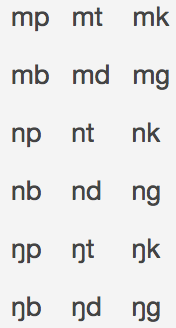
\includegraphics{../images/quiz4question5_a.png}
\end{figure}

~\\
INSTRUCTOR NOTES: contrast


~\\

{\large Question 2} (completed -nodate-) - Source: \\

What phonological relationships does this example show among the sounds [m], [n], and [ŋ], and why?\\

\begin{figure}[H]
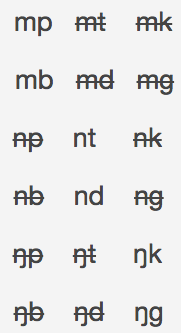
\includegraphics{../images/quiz4question5_b.png}
\end{figure}

~\\
INSTRUCTOR NOTES: allophony


~\\

{\large Question 3} (completed -nodate-) - Source: \\

What phonological relationships does this example show among the sounds [m], [n], and [ŋ], and why?\\

\begin{figure}[H]
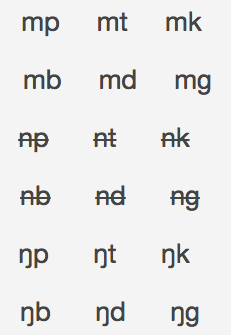
\includegraphics{../images/quiz4question5_c.png}
\end{figure}

~\\
INSTRUCTOR NOTES: contrast for [m] and [ŋ], but [n] doesn't occur


~\\

{\large Question 4} (completed -nodate-) - Source: \\

What phonological relationships does this example show among the sounds [m], [n], and [ŋ], and why?\\

\begin{figure}[H]
\includegraphics{../images/quiz4question5_d.png}
\end{figure}

~\\
INSTRUCTOR NOTES: contrast (with a few neutralizations)


~\\

{\large Question 5} (completed -nodate-) - Source: \\

Why should the following two questions have the same answer?\\

\begin{itemize} \item Given the vowel system of Jita, how many bi-syllabic root types would you expect to find for nouns in the language? \item Assuming that the vowel inventory is the same in verbs as it is in nouns, how many bisyllabic root types would you expect to find for verbs in the language? \end{itemize}


~\\
INSTRUCTOR NOTES: 


~\\

{\large Question 6} (completed -nodate-) - Source: \\

Explain how you would determine the phonological relationship between these two sounds (given below) in this dataset.\\

{[pʰ]} and {[f]}

\begin{figure}[H]
\includegraphics{../images/english_labials.png}
\end{figure}

~\\
INSTRUCTOR NOTES: contrastive; minimal pair


~\\

{\large Question 7} (completed -nodate-) - Source: \\

Explain how you would determine the phonological relationship between these two sounds (given below) in this dataset.\\

{[pʰ]} and {[p̚]}

\begin{figure}[H]
\includegraphics{../images/english_labials.png}
\end{figure}

~\\
INSTRUCTOR NOTES: free variation; pronunciation variants


~\\

{\large Question 8} (completed -nodate-) - Source: \\

Explain how you would determine the phonological relationship between these two sounds (given below) in this dataset.\\

{[l]} and {[ɾ]}

\begin{figure}[H]
\includegraphics{../images/korean.png}
\end{figure}

~\\
INSTRUCTOR NOTES: allophonic; complementary distribution


~\\

{\large Question 9} (completed -nodate-) - Source: \\

Explain how you would determine the phonological relationship between these two sounds (given below) in this dataset.\\

{[m]} and {[n]}

\begin{figure}[H]
\includegraphics{../images/canadianfrench.png}
\end{figure}

~\\
INSTRUCTOR NOTES: contrastive; [mu] ‘soft’ vs. [nu] ‘we’


~\\

{\large Question 10} (completed -nodate-) - Source: \\

Explain how you would determine the phonological relationship between these two sounds (given below) in this dataset.\\

{[f]} and {[v]}

\begin{figure}[H]
\includegraphics{../images/canadianfrench.png}
\end{figure}

~\\
INSTRUCTOR NOTES: contrastive; [fo] ‘false’ vs. [vo] ‘calf’


~\\

{\large Question 11} (completed -nodate-) - Source: \\

Explain how you would determine the phonological relationship between these two sounds (given below) in this dataset.\\

{[k]} and {[ɡ]}

\begin{figure}[H]
\includegraphics{../images/canadianfrench.png}
\end{figure}

~\\
INSTRUCTOR NOTES: contrastive; NEAR minimal pair; [evOk] ‘evoque’ vs. [vOg] ‘fashion’


~\\

{\large Question 12} (completed -nodate-) - Source: \\

Explain how you would determine the phonological relationship between these two sounds (given below) in this dataset.\\

{[d]} and {[n]}

\begin{figure}[H]
\includegraphics{../images/canadianfrench.png}
\end{figure}

~\\
INSTRUCTOR NOTES: contrastive; [do~] ‘donation’ vs. [no~] ‘no’


~\\

{\large Question 13} (completed -nodate-) - Source: \\

Explain how you would determine the phonological relationship between these two sounds (given below) in this dataset.\\

{[s]} and {[z]}

\begin{figure}[H]
\includegraphics{../images/canadianfrench.png}
\end{figure}

~\\
INSTRUCTOR NOTES: contrastive; [asyr] ‘assure’ vs. [azyr] ‘azure’


~\\

{\large Question 14} (completed -nodate-) - Source: \\

Explain how you would determine the phonological relationship between these two sounds (given below) in this dataset.\\

{[o]} and {[õ]}

\begin{figure}[H]
\includegraphics{../images/canadianfrench.png}
\end{figure}

~\\
INSTRUCTOR NOTES: contrastive; [do~] ‘donation’ vs. [do] ‘back’


~\\

{\large Question 15} (completed -nodate-) - Source: \\

Explain how you would determine the phonological relationship between these two sounds (given below) in this dataset.\\

{[l]} and {[ɫ]}

\begin{figure}[H]
\includegraphics{../images/english_laterals.png}
\end{figure}

~\\
INSTRUCTOR NOTES: [l] and [l̴] are allophonic in English. They are in complementary distribution, with [l] occurring before a vowel as in [lif] ‘leaf’ and [slɪm] ‘slim’ (and never after a vowel), and [l̴] occurring after a vowel, as in [fiɫ] ‘feel’ and [kɑɫd] ‘called’ (and never before a vowel).


~\\

{\large Question 16} (completed -nodate-) - Source: \\

Is the statement given below a good description of the distribution of sounds in this dataset? Why or why not?\\

The sounds {[pʰ]} and {[f]} are in complementary distribution. {[pʰ]} occurs after low vowels, as in {[kæpʰ]} ‘cap,’ while {[f]} occurs after high vowels, as in {[lif]} ‘leaf.’

\begin{figure}[H]
\includegraphics{../images/english_labials.png}
\end{figure}

~\\
INSTRUCTOR NOTES: no; the sounds are contrastive because there are minimal pairs, even though the example given isn't one


~\\

{\large Question 17} (completed -nodate-) - Source: \\

Is the statement given below a good description of the distribution of sounds in this dataset? Why or why not?\\

The sounds {[pʰ]} and {[p̚]} are in complementary distribution. {[pʰ]} occurs after front vowels, as in {[kæpʰ]} ‘cap,’ while {[p̚]} occurs after back vowels, as in {[tʃɑp̚]} ‘chop.’

\begin{figure}[H]
\includegraphics{../images/english_labials.png}
\end{figure}

~\\
INSTRUCTOR NOTES: no; the sounds are in free variation, because they can be variants of the same word, even though the example given doesn't show this


~\\

{\large Question 18} (completed -nodate-) - Source: \\

Is the statement given below a good description of the distribution of sounds in this dataset? Why or why not?\\

The sounds {[l]} and {[ɾ]} are in overlapping distribution. They can both occur after {[u]}, as in {[mul]} ‘water’ and {[muɾe]} ‘at the water.’ Thus, we know that these sounds are contrastive.

\begin{figure}[H]
\includegraphics{../images/korean.png}
\end{figure}

~\\
INSTRUCTOR NOTES: no; the sounds are allophonic, because the following environment is never the same


~\\

{\large Question 19} (completed -nodate-) - Source: \\

Is the statement given below a good description of the distribution of sounds in this dataset? Why or why not?\\

The sounds {[l]} and {[ɾ]} are in overlapping distribution, but just occur as pronunciation variants of the same morpheme, as in {[mul]} ‘water’ and {[muɾe]} ‘at the water.’ Thus, we know that these sounds are in free variation.

\begin{figure}[H]
\includegraphics{../images/korean.png}
\end{figure}

~\\
INSTRUCTOR NOTES: no; the sounds are allophonic, because the words are not actually identical -- these have different phonological contexts


~\\

{\large Question 20} (completed -nodate-) - Source: \\

Is the statement given below a good description of the distribution of sounds in this dataset? Why or why not?\\

The sounds {[l]} and {[ɫ]} are in complementary distribution. {[l]} occurs in onset position (before a vowel), but it becomes {[ɫ]} when it occurs in coda position (after a vowel).

\begin{figure}[H]
\includegraphics{../images/english_laterals.png}
\end{figure}

~\\
INSTRUCTOR NOTES: no; "becomes" is analytical, not descriptive


~\\

{\large Question 21} (completed -nodate-) - Source: \\

Is the statement given below a good description of the distribution of sounds in this dataset? Why or why not?\\

The sounds {[l]} and {[ɫ]} are in complementary distribution. {[ɫ]} occurs in coda position (after a vowel), but it turns into {[l]} when it occurs in onset position (before a vowel).

\begin{figure}[H]
\includegraphics{../images/english_laterals.png}
\end{figure}

~\\
INSTRUCTOR NOTES: no; "turns into" is analytical, not descriptive


~\\

{\large Question 22} (completed -nodate-) - Source: \\

State what kind of phonological relationship is shown between the sounds [o] and [a] and explain how you know.\\

\begin{figure}[H]
\includegraphics{../images/peng70ao_a.png}
\end{figure}

~\\
INSTRUCTOR NOTES: contrast (both occur after [i], [u], [a], and neither occurs after [o]); some neutralization in that [o] can't occur before [a] or [o], but [a] can


~\\

{\large Question 23} (completed -nodate-) - Source: \\

State what kind of phonological relationship is shown between the sounds [o] and [a] and explain how you know.\\

\begin{figure}[H]
\includegraphics{../images/peng70ao_b.png}
\end{figure}

~\\
INSTRUCTOR NOTES: contrast (both occur after [u], [o], [a] and before [o], [a]); neutralized after [i]


~\\

{\large Question 24} (completed -nodate-) - Source: \\

State what kind of phonological relationship is shown between the sounds [o] and [a] and explain how you know.\\

\begin{figure}[H]
\includegraphics{../images/peng70ao_c.png}
\end{figure}

~\\
INSTRUCTOR NOTES: allophony; [o] occurs only next to [o], and [a] occurs nect to any other vowel but not [o]


~\\

{\large Question 25} (completed -nodate-) - Source: \\

State what kind of phonological relationship is shown between the sounds [o] and [a] and explain how you know.\\

\begin{figure}[H]
\includegraphics{../images/peng70ao_d.png}
\end{figure}

~\\
INSTRUCTOR NOTES: contrast (both can occur everywhere -- no neutralization)


~\\

{\large Question 26} (completed -nodate-) - Source: \\

Explain whether the rule below would apply to the form shown, and if so, what the effect of the rule would be. Assume the vowel inventory [i], [ɪ], [e], [ɛ], [ɑ], [u], [ʊ], [o], [ɔ].\\

/isɪm/

{[high vowel]} →  {[unround, front]} / {[front vowel]} C$_0$ \_\_ 


~\\
INSTRUCTOR NOTES: applies; no effect


~\\

{\large Question 27} (completed -nodate-) - Source: \\

Explain whether the rule below would apply to the form shown, and if so, what the effect of the rule would be. Assume the vowel inventory [i], [ɪ], [e], [ɛ], [ɑ], [u], [ʊ], [o], [ɔ].\\

/ʊsɔm/

{[high vowel]} →  {[unround, front]} / {[front vowel]} C$_0$ \_\_ 


~\\
INSTRUCTOR NOTES: doesn't apply


~\\

{\large Question 28} (completed -nodate-) - Source: \\

Explain whether the rule below would apply to the form shown, and if so, what the effect of the rule would be. Assume the vowel inventory [i], [ɪ], [e], [ɛ], [ɑ], [u], [ʊ], [o], [ɔ].\\

/emɛs/

{[high vowel]} →  {[unround, front]} / {[front vowel]} C$_0$ \_\_ 


~\\
INSTRUCTOR NOTES: doesn't apply


~\\

{\large Question 29} (completed -nodate-) - Source: \\

Explain whether the rule below would apply to the form shown, and if so, what the effect of the rule would be. Assume the vowel inventory [i], [ɪ], [e], [ɛ], [ɑ], [u], [ʊ], [o], [ɔ].\\

/emus/

{[high vowel]} →  {[unround, front]} / {[front vowel]} C$_0$ \_\_ 


~\\
INSTRUCTOR NOTES: applies; [emis]


~\\

{\large Question 30} (completed -nodate-) - Source: \\

Explain whether the rule below would apply to the form shown, and if so, what the effect of the rule would be. Assume the vowel inventory [i], [ɪ], [e], [ɛ], [ɑ], [u], [ʊ], [o], [ɔ].\\

/emos/

{[high vowel]} →  {[unround, front]} / {[front vowel]} C$_0$ \_\_ 


~\\
INSTRUCTOR NOTES: doesn't apply


~\\

{\large Question 31} (completed -nodate-) - Source: \\

Explain whether the rule below would apply to the form shown, and if so, what the effect of the rule would be. Assume the vowel inventory [i], [ɪ], [e], [ɛ], [ɑ], [u], [ʊ], [o], [ɔ].\\

/imɑm/

{[high vowel]} →  {[unround, front]} / {[front vowel]} C$_0$ \_\_ 


~\\
INSTRUCTOR NOTES: doesn't apply


~\\

{\large Question 32} (completed -nodate-) - Source: \\

Explain whether the rule below would apply to the form shown, and if so, what the effect of the rule would be. Assume the vowel inventory [i], [ɪ], [e], [ɛ], [ɑ], [u], [ʊ], [o], [ɔ].\\

/isɪm/

{[non-low vowel]} →  {[lax]} / \_\_ C$_0$ {[lax vowel]}


~\\
INSTRUCTOR NOTES: applies; [ɪsɪm]


~\\

{\large Question 33} (completed -nodate-) - Source: \\

Explain whether the rule below would apply to the form shown, and if so, what the effect of the rule would be. Assume the vowel inventory [i], [ɪ], [e], [ɛ], [ɑ], [u], [ʊ], [o], [ɔ].\\

/ʊsɔm/

{[non-low vowel]} →  {[lax]} / \_\_ C$_0$ {[lax vowel]}


~\\
INSTRUCTOR NOTES: applies; no effect


~\\

{\large Question 34} (completed -nodate-) - Source: \\

Explain whether the rule below would apply to the form shown, and if so, what the effect of the rule would be. Assume the vowel inventory [i], [ɪ], [e], [ɛ], [ɑ], [u], [ʊ], [o], [ɔ].\\

/emɛs/

{[non-low vowel]} →  {[lax]} / \_\_ C$_0$ {[lax vowel]}


~\\
INSTRUCTOR NOTES: applies; [ɛmɛs]


~\\

{\large Question 35} (completed -nodate-) - Source: \\

Explain whether the rule below would apply to the form shown, and if so, what the effect of the rule would be. Assume the vowel inventory [i], [ɪ], [e], [ɛ], [ɑ], [u], [ʊ], [o], [ɔ].\\

/emus/

{[non-low vowel]} →  {[lax]} / \_\_ C$_0$ {[lax vowel]}


~\\
INSTRUCTOR NOTES: doesn't apply


~\\

{\large Question 36} (completed -nodate-) - Source: \\

Explain whether the rule below would apply to the form shown, and if so, what the effect of the rule would be. Assume the vowel inventory [i], [ɪ], [e], [ɛ], [ɑ], [u], [ʊ], [o], [ɔ].\\

/emos/

{[non-low vowel]} →  {[lax]} / \_\_ C$_0$ {[lax vowel]}


~\\
INSTRUCTOR NOTES: doesn't apply


~\\

{\large Question 37} (completed -nodate-) - Source: \\

Explain whether the rule below would apply to the form shown, and if so, what the effect of the rule would be. Assume the vowel inventory [i], [ɪ], [e], [ɛ], [ɑ], [u], [ʊ], [o], [ɔ].\\

/imɑm/

{[non-low vowel]} →  {[lax]} / \_\_ C$_0$ {[lax vowel]}


~\\
INSTRUCTOR NOTES: doesn't apply (unless [ɑ] treated as lax)


~\\

{\large Question 38} (completed -nodate-) - Source: \\

Explain how you would choose the underlying representation of the phoneme with allophones [s] and [ʃ].\\

\begin{figure}[H]
\includegraphics{../images/japanese.png}
\end{figure}

~\\
INSTRUCTOR NOTES: We would probably pick the alveolar version /s/ to be the underlying representation, because it occurs in a wider set of contexts. That way, we can write a single rule to derive the more limited distribution of the palatal, and not need rules to explain any of alveolar occurrences.


~\\

{\large Question 39} (completed -nodate-) - Source: \\

Explain how you would choose the underlying representation of the phoneme with allophones [z] and [dʒ].\\

\begin{figure}[H]
\includegraphics{../images/japanese.png}
\end{figure}

~\\
INSTRUCTOR NOTES: We would probably pick the alveolar version /z/ to be the underlying representation, because it occurs in a wider set of contexts. That way, we can write a single rule to derive the more limited distribution of the palatal, and not need rules to explain any of alveolar occurrences.


~\\

{\large Question 40} (completed -nodate-) - Source: \\

Explain how you would choose the underlying representation for the phoneme with allophones [ʊ] and [ɯ].\\

\begin{figure}[H]
\includegraphics{../images/tamil.png}
\end{figure}

~\\
INSTRUCTOR NOTES: The phoneme category should be /ʊ/, because it occurs in the wider range of situations – especially when there is no preceding vowel that would condition whether it should be rounded or not. That is, it seems to the be “default” vowel.


\newpage\textbf{\underline{\huge Phonological Relationships and Analysis / very hard\\}}

~\\

{\large Question 1} (completed -nodate-) - Source: \\

What do the two signs below tell you about the phonological status of \underline{handshape} in ASL, and why?\\

\begin{figure}[H]
\includegraphics{../images/asl_apple.png}
\caption{APPLE}
\end{figure}
\begin{figure}[H]
\includegraphics{../images/asl_candy.png}
\caption{CANDY}
\end{figure}

~\\
INSTRUCTOR NOTES: shows contrast because movement and location are same


~\\

{\large Question 2} (completed -nodate-) - Source: \\

What do the two signs below tell you about the phonological status of \underline{handshape} in ASL, and why?\\

\begin{figure}[H]
\includegraphics{../images/asl_stay.png}
\caption{STAY}
\end{figure}
\begin{figure}[H]
\includegraphics{../images/asl_awkward.png}
\caption{AWKWARD}
\end{figure}

~\\
INSTRUCTOR NOTES: nothing, because both handshape and movement are different


~\\

{\large Question 3} (completed -nodate-) - Source: \\

What do the two signs below tell you about the phonological status of \underline{handshape} in ASL, and why?\\

\begin{figure}[H]
\includegraphics{../images/asl_apple.png}
\caption{APPLE}
\end{figure}
\begin{figure}[H]
\includegraphics{../images/asl_now.png}
\caption{NOW}
\end{figure}

~\\
INSTRUCTOR NOTES: nothing, because handshape and location and movement are all also different


~\\

{\large Question 4} (completed -nodate-) - Source: \\

What is the basic analysis of vowel length in this dataset, and what are the key pieces of evidence?\\

\begin{figure}[H]
\includegraphics{../images/malayalam.png}
\end{figure}

~\\
INSTRUCTOR NOTES: Short and long vowels appear to be contrastive (phonemic) in Malayalam, as evidenced by minimal pairs that differ only in terms of their vowel length, such as [koʈːa] ‘basket’ vs. [koːʈːa] ‘castle’ or [keʈːu] ‘burnt out’ vs. [keːʈːu] ‘heard.’


~\\

{\large Question 5} (completed -nodate-) - Source: \\

What is the basic analysis of voiceless stops in this dataset, and what are the key pieces of evidence?\\

\begin{figure}[H]
\includegraphics{../images/english11.png}
\end{figure}

~\\
INSTRUCTOR NOTES: Plain and aspirated voiceless stops are in complementary distribution in English. Plain stops occur always and only after [s], as in [speɪs] ‘space,’ while aspirated stops never occur in this context. Meanwhile, aspirated stops occur word-initially (e.g., [phitʃ] ‘peach’) and between vowels (e.g., [əphɑɹt] ‘apart’). Because the two are in complementary distribution, we can always predict which one occurs in any given environment, and so we conclude that they are allophonic, i.e., allophones of the same phoneme category. 


~\\

{\large Question 6} (completed -nodate-) - Source: \\

What is the basic analysis of oral and nasal vowels in this dataset, and what are the key pieces of evidence?\\

\begin{figure}[H]
\includegraphics{../images/english12.png}
\end{figure}

~\\
INSTRUCTOR NOTES: The pairs of sounds [i] and [ĩ], and [u] and [ũ], are each allophonic and therefore allophones of the same phoneme in English (though the two pairs represent two contrastive phonemes in English). The sounds [i] and [ĩ] are in complementary distribution in English, with [ĩ] occurring before the sounds [m] and [n], (e.g., [ɡlĩm] ‘gleam’ and [klĩn] ‘clean’) and [i] occurring elsewhere (e.g., [lip] ‘leap’). Similarly, the sounds [u] and [ũ] are also in complementary distribution, with exactly the same conditioning environments: [ũ] occurs before [m] and [n] (e.g., [dũm] ‘doom’ and [dũn] ‘dune’), and [u] occurs elsewhere (e.g. [but] ‘boot’). Thus, within each pair, we treat the vowels as allophonic. 


\newpage\textbf{\underline{\huge Phonological Relationships and Analysis / easy\\}}

~\\

{\large Question 1} (completed -nodate-) - Source: \\

Explain why the statement below either is or is not a good analysis of the data.\\

Because {[r]} and {[r̥]} are contrastive in English, we cannot write a rule to account for their distribution.

\begin{figure}[H]
\includegraphics{../images/peng71_englishr.png}
\end{figure}

~\\
INSTRUCTOR NOTES: not a good analysis because the two sounds are in complementary distribution


~\\

{\large Question 2} (completed -nodate-) - Source: \\

Explain why the statement below either is or is not a good analysis of the data.\\

We should posit /r/ as the underlying form, and have a rule that devoices it when it occurs after voiceless segments. This analysis is best because it requires only one rule with a single environment to account for all the occurrences of both {[r]} and {[r̥]}; the plain {[r]} sounds result from non-application of the rule.

\begin{figure}[H]
\includegraphics{../images/peng71_englishr.png}
\end{figure}

~\\
INSTRUCTOR NOTES: a good analysis


~\\

{\large Question 3} (completed -nodate-) - Source: \\

Explain why the statement below either is or is not a good analysis of the data.\\

We should posit /r̥/ as the underlying form, and have a rule that voices it when it occurs after voiced segments or word-initially. This analysis is best because it puts the more unusual sound, the voiceless {[r̥]}, into the underlying representation, which has to be memorized anyway.

\begin{figure}[H]
\includegraphics{../images/peng71_englishr.png}
\end{figure}

~\\
INSTRUCTOR NOTES: not a good analysis, because we want the UR to occur in the MOST environments, not the FEWEST (makes the rule simpler)


~\\

{\large Question 4} (completed -nodate-) - Source: \\

Explain why the statement below either is or is not a good analysis of the data.\\

Because {[r]} and {[r̥]} are in free variation in English, we cannot write a rule to account for their distribution.

\begin{figure}[H]
\includegraphics{../images/peng71_englishr.png}
\end{figure}

~\\
INSTRUCTOR NOTES: not a good analysis, because the sounds are in complementary distribution


~\\

{\large Question 5} (completed -nodate-) - Source: \\

Explain what the rule below does and suggest a name for it, explaining why that would be a good name.\\

/n/ → {[m]} / \_\_ \{{[p]}, {[b]}\}


~\\
INSTRUCTOR NOTES: 


~\\

{\large Question 6} (completed -nodate-) - Source: \\

Explain what the rule below does and suggest a name for it, explaining why that would be a good name.\\

/n/ → {[ŋ]} / \_\_ {[velar]}


~\\
INSTRUCTOR NOTES: 


~\\

{\large Question 7} (completed -nodate-) - Source: \\

Explain what the rule below does and suggest a name for it, explaining why that would be a good name.\\

{[nasal]} → {[αPlace]} / \_\_ {[αPlace]}


~\\
INSTRUCTOR NOTES: 


~\\

{\large Question 8} (completed -nodate-) - Source: \\

Explain what the rule below does and suggest a name for it, explaining why that would be a good name.\\

{[vowel]} → {[nasal]} / {[nasal]} \_\_


~\\
INSTRUCTOR NOTES: 


~\\

{\large Question 9} (completed -nodate-) - Source: \\

Explain what the rule below does and suggest a name for it, explaining why that would be a good name.\\

{[high vowel]} →  {[unround, front]} / {[front vowel]} C$_0$ \_\_


~\\
INSTRUCTOR NOTES: 


~\\

{\large Question 10} (completed -nodate-) - Source: \\

Explain what the rule below does and suggest a name for it, explaining why that would be a good name.\\

{[non-low vowel]} →  {[lax]} / \_\_ C$_0$ {[lax vowel]}


~\\
INSTRUCTOR NOTES: 


\newpage\textbf{\underline{\huge Acoustics / hard\\}}

~\\

{\large Question 1} (completed -nodate-) - Source: \\

Explain what you see in the spectrogram that tells you about the properties of the sounds in the pictured word.\\

\begin{figure}[H]
\includegraphics{../images/spectrogram_shoe.png}
\end{figure}

~\\
INSTRUCTOR NOTES: shoe: fricative noise at mid-frequency; no voice bar; vowel formants that suggest low F1 (high V) and low F2 (back V)


~\\

{\large Question 2} (completed -nodate-) - Source: \\

Explain what you see in the spectrogram that tells you about the properties of the sounds in the pictured word.\\

\begin{figure}[H]
\includegraphics{../images/spectrogram_hippo.png}
\end{figure}

~\\
INSTRUCTOR NOTES: hippo: stop in middle indicated by silence / white space; vowels on either side; V1 has low F1 and high F2 (=high front V) and V2 has higher F1 and lower F2 (=mid to low backer vowel)


~\\

{\large Question 3} (completed -nodate-) - Source: \\

Explain what you see in the spectrogram that tells you about the properties of the sounds in the pictured word.\\

\begin{figure}[H]
\includegraphics{../images/spectrogram_aaah.png}
\end{figure}

~\\
INSTRUCTOR NOTES: aaah: just a vowel; formants are very steady; F1 and F2 are pretty close to each other; F1 somewhat high and F2 somewhat low


~\\

{\large Question 4} (completed -nodate-) - Source: \\

Explain what you see in the spectrogram that tells you about the properties of the sounds in the pictured word.\\

\begin{figure}[H]
\includegraphics{../images/spectrogram_you.png}
\end{figure}

~\\
INSTRUCTOR NOTES: you: clear formants, but starts with something like a glide because fainter; diphthong or changing values; F1 pretty constantly low (=high V); F2 starts high and goes low (=front to back)


~\\

{\large Question 5} (completed -nodate-) - Source: \\

Explain what you see in the spectrogram that tells you about the properties of the sounds in the pictured word.\\

\begin{figure}[H]
\includegraphics{../images/spectrogram_I.png}
\end{figure}

~\\
INSTRUCTOR NOTES: I: clear formants; all dark, so just a vowel; changes so a diphthong; F1 pretty high and then falls a bit (=starts as low V and goes higher); F2 starts pretty low and then goes up (=starts as back V and goes fronter)


~\\

{\large Question 6} (completed -nodate-) - Source: \\

Explain what you see in the spectrogram that tells you about the properties of the sounds in the pictured word.\\

\begin{figure}[H]
\includegraphics{../images/spectrogram_oh.png}
\end{figure}

~\\
INSTRUCTOR NOTES: oh: just a vowel; clear formants; pretty steady with a slight downward trend of both; F1 is pretty close to F2, which means F2 is pretty low (=back V), and F1 isn't super low (=mid to low vowel)


~\\

{\large Question 7} (completed -nodate-) - Source: \\

Explain what you see in the spectrogram that tells you about the properties of the sounds in the pictured word.\\

\begin{figure}[H]
\includegraphics{../images/spectrogram_we.png}
\end{figure}

~\\
INSTRUCTOR NOTES: we: starts paler, then darker, so glide plus vowel; F1 pretty constantly low (=high V); F2 starts very low and then swoops up (=starts back and goes front)


~\\

{\large Question 8} (completed -nodate-) - Source: \\

Explain what you see in the spectrogram that tells you about the properties of the sounds in the pictured word.\\

\begin{figure}[H]
\includegraphics{../images/spectrogram_suit.png}
\end{figure}

~\\
INSTRUCTOR NOTES: suit: starts with fricative noise; then some kind of vowel; then a stop with a release burst; fricative is voiceless (no voice bar); fricative likely [s] because high-energy; vowel has low F1 (=high V) but then hard to see F2; stop is also voiceless


~\\

{\large Question 9} (completed -nodate-) - Source: \\

Briefly explain source-filter theory.\\


~\\
INSTRUCTOR NOTES: The vocal folds vibrate, setting the air coming from the lungs into motion -- this is the "source" sound wave, which is a complex wave, with energy at multiple different frequencies – the fundamental and its harmonics, i.e., its multiples. Then the oral and nasal cavities act as a "filter" to dampen (remove energy from) some of the frequencies of the sound and enhance others (the resonant frequencies). Depending on the shape of the mouth, different frequencies will resonate and so we get different formant values and hence different vowel qualities.


\newpage\textbf{\underline{\huge Acoustics / easy\\}}

~\\

{\large Question 1} (completed -nodate-) - Source: \\

Explain what (if anything) the letter below represents on this waveform.\\

A

\begin{figure}[H]
\includegraphics{../images/sinusoid.png}
\end{figure}

~\\
INSTRUCTOR NOTES: wavelength or period


~\\

{\large Question 2} (completed -nodate-) - Source: \\

Explain what (if anything) the letter below represents on this waveform.\\

B

\begin{figure}[H]
\includegraphics{../images/sinusoid.png}
\end{figure}

~\\
INSTRUCTOR NOTES: nothing (twice amplitude)


~\\

{\large Question 3} (completed -nodate-) - Source: \\

Explain what (if anything) the letter below represents on this waveform.\\

C

\begin{figure}[H]
\includegraphics{../images/sinusoid.png}
\end{figure}

~\\
INSTRUCTOR NOTES: nothing (half wavelength or half period)


~\\

{\large Question 4} (completed -nodate-) - Source: \\

Explain what (if anything) the letter below represents on this waveform.\\

D

\begin{figure}[H]
\includegraphics{../images/sinusoid.png}
\end{figure}

~\\
INSTRUCTOR NOTES: amplitude


~\\

{\large Question 5} (completed -nodate-) - Source: \\

Explain what (if anything) the letter below represents on this waveform.\\

E

\begin{figure}[H]
\includegraphics{../images/sinusoid.png}
\end{figure}

~\\
INSTRUCTOR NOTES: nothing (half wavelength or half period)


\newpage\textbf{\underline{\huge Acoustics / medium\\}}

~\\

{\large Question 1} (completed -nodate-) - Source: \\

Explain how each component of the description below gives you information about the sound being described.\\

This consonant is characterized by having the adjacent second and third formants “pinched” together; that is, F3 moves down and F2 moves up if you go from a vowel into this consonant. There is often a clear voice bar, but there’s no evidence of formants in the consonant itself. In fact, there’s not much energy during the consonant at all.


~\\
INSTRUCTOR NOTES: [ɡ]; check for voicing, place, and manner


~\\

{\large Question 2} (completed -nodate-) - Source: \\

Explain how each component of the description below gives you information about the sound being described.\\

This consonant is characterized by having a clear voice bar and its own formants (at around 250 Hz, 2500 Hz, and 3250 Hz). These formants, however, are not as intense as they would be if they were vowel formants. The effect on the formants of the adjacent vowel is usually relatively small; the second formant of the vowel will probably be around 1750 Hz.


~\\
INSTRUCTOR NOTES: [n]; check for voicing, place, and manner


~\\

{\large Question 3} (completed -nodate-) - Source: \\

Explain how each component of the description below gives you information about the sound being described.\\

This consonant is characterized by having a lot of random noise in the spectrogram, with no clear formant structure at all. It tends to be longer and louder than other similar consonants. There is no voice bar, and the majority of the noise created by this consonant is at relatively high frequencies.


~\\
INSTRUCTOR NOTES: [s]; check for voicing, place, and manner


~\\

{\large Question 4} (completed -nodate-) - Source: \\

Explain how each component of the description below gives you information about the sound being described.\\

This consonant typically starts off with nothing at all visible on the spectrogram. There is then a short period of noise between the silence and the following vowel. This consonant typically brings the second and third formants of the adjacent vowel down.


~\\
INSTRUCTOR NOTES: [pʰ]; check for voicing, place, and manner


~\\

{\large Question 5} (completed -nodate-) - Source: \\

Explain why each numbered, underlined statement is true or false. If it is false, explain one way that you could correct it.\\

Sound is an invisible phenomenon. Sound can travel through any substance, $^1$\ul{such as a liquid, solid, or a gas.} $^2$\ul{It involves the transfer of the matter in that substance} from one place to another.\\\\Sound is a particular kind of wave known as $^3$\ul{a compression wave}. $^4$\ul{When the molecules are really close together, we say they are ``rarefied'' and when they are really far apart, we say they are ``compressed.''}


~\\
INSTRUCTOR NOTES: 1 - true.\\2 - false (it involves the transfer of energy... or anything about the matter itself not moving but only vibrating, etc). \\3 - true.\\4 - false (when the molecules are really close together, we say they are compressed and when the molecules are really far apart, we say they are rarefied).


~\\

{\large Question 6} (completed -nodate-) - Source: \\

Explain why each numbered, underlined statement is true or false. If it is false, explain one way that you could correct it.\\

Sound is a particular kind of wave known as a compression wave.... $^6$\ul{When the molecules are really close together, they try to spread out as far as possible, and that’s why they move out as a wave.}\\\\There are several key components of a sound wave. The first is wavelength. $^7$\ul{Wavelength is the distance between the point of maximum rarefaction and the point of maximum compression in a wave.} Another component that is related to wavelength is $^8$\ul{frequency, or how many times a wave passes through a particular point in one second.} $^9$\ul{If the wavelength is really short, the frequency will be really high; if the wavelength is really long, the frequency will be really low.} 


~\\
INSTRUCTOR NOTES: 6 - false (the molecules always try to stay an equal distance from each other, so they move apart when they are compressed and together when they are rarefied).\\7 - false (wavelength is the distance between two points of maximum compression or rarefaction in a wave).\\8 - true.\\9 - true.


~\\

{\large Question 7} (completed -nodate-) - Source: \\

Explain why each numbered, underlined statement is true or false. If it is false, explain one way that you could correct it.\\

$^{10}$\ul{Frequency is inversely related to pitch: high frequencies correspond to low pitches, and low frequencies correspond to high pitches.} Finally, there is the amplitude of the wave. $^{11}$\ul{The amplitude tells you how much pressure the molecules are under at any particular time.} $^{12}$\ul{The auditory correlate of amplitude is intensity}; this is a measure of perceived pressure.\\\\$^{13}$\ul{In speech, air is set in vibrating motion by the lungs, so the lungs} are the source of most speech sounds.


~\\
INSTRUCTOR NOTES: 10 - false (frequency is directly related to pitch: high frequencies correspond to high pitches, and low frequencies correspond to low pitches).\\11 - true.\\12 - false (the auditory correlate of amplitude and intensity is loudness/volume, or, a related acoustic measure to amplitude is intensity).\\13 - false (air is set in vibrating motion by the vocal folds).


~\\

{\large Question 8} (completed -nodate-) - Source: \\

Explain why each numbered, underlined statement is true or false. If it is false, explain one way that you could correct it.\\

In speech, air is set in vibrating motion by the lungs, so the lungs are the source of most speech sounds. $^{14}$\ul{The basic rate of vibration is called the fundamental frequency}; $^{15}$\ul{the fundamental frequency is also known as the timbre of the voice.} In addition to the source, we can also talk about a filter: $^{16}$\ul{the vocal folds act as a filter to shape the air from the lungs into the sounds we hear as different.} $^{17}$\ul{The mouth and nose act as resonance chambers}, and these also affect the qualities of the sounds.


~\\
INSTRUCTOR NOTES: 14 - true.\\15 - false (the fundamental frequency is also known as the pitch of the voice, or F0).\\16 - false (the mouth and nose act as a filter to shape the air from the vocal folds in the sounds we hear as different, or vocal tract, or articulatory and resonance chambers, etc).\\17 - true.


~\\

{\large Question 9} (completed -nodate-) - Source: \\

Explain why each numbered, underlined statement is true or false. If it is false, explain one way that you could correct it.\\

We can visualize speech through the use of spectra and spectrograms. $^{18}$\ul{A spectrogram shows frequency on the horizontal axis and amplitude on the vertical axis.} $^{19}$\ul{A spectrum, on the other hand, shows frequency on the vertical axis and time along the horizontal axis}.\\\\$^{20}$\ul{On a spectrogram, the dark bars are called formants.} $^{21}$\ul{The formants correspond to the amplitude peaks on a spectrum.}


~\\
INSTRUCTOR NOTES: 18 - false (A spectrum shows frequency on the horizontal axis and amplitude on the vertical axis, or, a spectrogram shows frequency on the vertical axis and time along the horizontal axis).\\19 - false (A spectrum shows frequency on the horizontal axis and amplitude on the vertical axis, or, a spectrogram shows frequency on the vertical axis and time along the horizontal axis).\\20 - true.\\21 - true.


~\\

{\large Question 10} (completed -nodate-) - Source: \\

Explain why each numbered, underlined statement is true or false. If it is false, explain one way that you could correct it.\\

We can look at the vertical location of the formants to determine something about the characteristics of individual speech sounds. For example, in the two spectrograms below, we can see that $^{22}$\ul{the first formant is higher in the spectrogram for sound 1 than it is for sound 2.} Because $^{23}$\ul{F1 is directly correlated with vowel height}, we know that $^{24}$\ul{the vowel pictured in sound 1 is a higher vowel than the one in sound 2}. For example, $^{25}$\ul{sound 1 might be an {[ɑ]} while sound 2 might be an {[i]}.}

\begin{figure}[H]
\includegraphics{../images/sound1a_sound2i.png}
\end{figure}

~\\
INSTRUCTOR NOTES: 22 - true. \\23 - false (F1 is inversely correlated with vowel height). \\24 - false (the vowel pictured in sound 1 is a lower vowel than the one in sound 2, or, the vowel pictured in sound 2 is a higher vowel than the one in sound 1).\\25 - true.


\newpage\textbf{\underline{\huge Alternations / medium\\}}

~\\

{\large Question 1} (completed -nodate-) - Source: \\

Based on this data from Lamba, explain why the pair given below either does or does not show that the consonants preceding the morpheme for `with' are NOT responsible for the variation between [-il] and [-el].\\

čit-a \& čit-il-a

\begin{figure}[H]
\includegraphics{../images/peng119_lamba.png}
\end{figure}

~\\
INSTRUCTOR NOTES: doesn't show this -- only the [il] form is shown, so we can't judge whether [il] ~ [el] is based on consonants or not


~\\

{\large Question 2} (completed -nodate-) - Source: \\

Based on this data from Lamba, explain why the pair given below either does or does not show that the consonants preceding the morpheme for `with' are NOT responsible for the variation between [-il] and [-el].\\

čet-el-a \& čit-il-a

\begin{figure}[H]
\includegraphics{../images/peng119_lamba.png}
\end{figure}

~\\
INSTRUCTOR NOTES: does show this -- we see both [il] and [el], and they occur after the SAME preceding consonant, so the preceding consonant cannot be responsible


~\\

{\large Question 3} (completed -nodate-) - Source: \\

Based on this data from Lamba, explain why the pair given below either does or does not show that the consonants preceding the morpheme for `with' are NOT responsible for the variation between [-il] and [-el].\\

tul-il-a \& soŋk-el-a

\begin{figure}[H]
\includegraphics{../images/peng119_lamba.png}
\end{figure}

~\\
INSTRUCTOR NOTES: doesn't show this -- we do see [il] and [el], but they occur after different consonants, so it COULD be the consonant that is responsible


~\\

{\large Question 4} (completed -nodate-) - Source: \\

Based on this data from Lamba, explain why the pair given below either does or does not show that the consonants preceding the morpheme for `with' are NOT responsible for the variation between [-il] and [-el].\\

pat-il-a \& tul-il-a

\begin{figure}[H]
\includegraphics{../images/peng119_lamba.png}
\end{figure}

~\\
INSTRUCTOR NOTES: doesn't show this -- we only see [il], so we don't know if [el] can also occur in these environments or not


~\\

{\large Question 5} (completed -nodate-) - Source: \\

Explain which morpheme(s) in this dataset alternate and how that helps you do a phonological analysis.\\

\begin{figure}[H]
\includegraphics{../images/english_past.png}
\end{figure}

~\\
INSTRUCTOR NOTES: the past tense morpheme alternates, so we know we need to analyze the predictable occurrence of [t] vs. [d]


~\\

{\large Question 6} (completed -nodate-) - Source: \\

Explain which morpheme(s) in this dataset alternate and how that helps you do a phonological analysis.\\

\begin{figure}[H]
\includegraphics{../images/japanese_verbs.png}
\end{figure}

~\\
INSTRUCTOR NOTES: each verb root alternates, so we know the sounds we need to analyze are the predictable occurrence of [s] and [ʃ]


~\\

{\large Question 7} (completed -nodate-) - Source: \\

Explain which morpheme(s) in this dataset alternate and how that helps you do a phonological analysis.\\

\begin{figure}[H]
\includegraphics{../images/english_t_flap.png}
\end{figure}

~\\
INSTRUCTOR NOTES: some of the roots alternate (such as 'light'), so we know that we need to analyze the predictable occurrence of [t] vs. [flap]


\newpage\textbf{\underline{\huge Alternations / easy\\}}

~\\

{\large Question 1} (completed -nodate-) - Source: \\

Explain why the concept of an alternation either is or is not useful for understanding this dataset.\\

\begin{figure}[H]
\includegraphics{../images/korean.png}
\end{figure}

~\\
INSTRUCTOR NOTES: is useful -- root morphemes alternate, so we can decide which sounds we need to analyze


~\\

{\large Question 2} (completed -nodate-) - Source: \\

Explain why the concept of an alternation either is or is not useful for understanding this dataset.\\

\begin{figure}[H]
\includegraphics{../images/osage.png}
\end{figure}

~\\
INSTRUCTOR NOTES: is not useful -- there are no alternations in this dataset, so we can't use them to figure out what sounds are relevant to analyse


~\\

{\large Question 3} (completed -nodate-) - Source: \\

Explain why what you’re analyzing in the following dataset either is or is not an alternation.\\

\begin{figure}[H]
\includegraphics{../images/yawelmani.png}
\end{figure}

~\\
INSTRUCTOR NOTES: it's not an alternation -- we don't have multiple *surface* forms of the same morpheme; the different forms are the UR and the SR, and so they are not predictable from phonological context (the SR is derived from the UR by rule)


\newpage\textbf{\underline{\huge Phonological Features / hard\\}}

~\\

{\large Question 1} (completed 20201002) - Source: Week 4 Discussion\\

Explain why phonological features are used instead of phonetic characteristics in analyzing datasets.\\


~\\
INSTRUCTOR NOTES: Phonological features help to capture phonological patterns, i.e., they group sounds together based on whether they do things like triggering a change or undergoing a change. Phonological features are sometimes language-specific. Phonetic characteristics are simply descriptions of the physical properties of the sounds; they are language-universal and independent of the patterns (though it turns out that many phonological patterns are based on phonetic characteristic groupings).


~\\

{\large Question 2} (completed 20200929) - Source: Quiz 3, Question 12\\

Explain how you figure out which feature is involved in the process of umlaut.\\

\begin{figure}[H]
\includegraphics{../images/dutch.png}
\end{figure}

~\\
INSTRUCTOR NOTES: we look to see which vowels are affected, and compare them to see which feature is DIFFERENT (not e.g. what features they share); so since the vowels in the singular and plural are identical except that the singular forms are back and the plural are front, it's the feature [back] that is relevant / changing / involved (not e.g. the feature [round] just because all of the vowels are round)


~\\

{\large Question 3} (completed -nodate-) - Source: \\

Explain how you should use phonological features to combine these rules.\\

/s/ → {[ʃ]} / \_\_ {[i]} \\/z/ → {[dʒ]} / \_\_ {[i]}

\begin{figure}[H]
\includegraphics{../images/japanese.png}
\end{figure}

~\\
INSTRUCTOR NOTES: input should be alveolar fricatives, output should be just a change in place of articulation; context is still [i]; something like [CORONAL, +strid] --> [-ant, +dist] / \_\_ [i]; note that this won't directly account for why the voiced one becomes an affricate


~\\

{\large Question 4} (completed -nodate-) - Source: \\

Explain how you should use phonological features in this rule. Which parts of the rule should include features, and which features should be used?\\

/ʊ/ → {[ɯ]} / {[unrounded vowel]} C$_0$ \_\_

\begin{figure}[H]
\includegraphics{../images/tamil.png}
\end{figure}

~\\
INSTRUCTOR NOTES: input can be just a segment; output should be [-round], context should be [-round, +syllabic]


~\\

{\large Question 5} (completed -nodate-) - Source: \\

Explain how you should use phonological features in this rule. Which parts of the rule should include features, and what features might they be? You don't have to give an exact set of features, but what kinds of features would be involved?\\

/ð/ → {[d]} / \_\_ {[a]}

\begin{figure}[H]
\includegraphics{../images/osage.png}
\end{figure}

~\\
INSTRUCTOR NOTES: input can be just a segment; output should be something like [-cont]; context can be a segment; this doesn't by itself account for the slight difference in place of articulation


~\\

{\large Question 6} (completed -nodate-) - Source: \\

Explain how you should use phonological features to combine these rules.\\

/pʰ/ → {[p]} / {[s]} \_\_\\/tʰ/ → {[t]} / {[s]} \_\_\\/kʰ/ → {[k]} / {[s]} \_\_

\begin{figure}[H]
\includegraphics{../images/english_asp.png}
\end{figure}

~\\
INSTRUCTOR NOTES: input should be aspirated voiceless stops; output should lose the aspiration; context can just be an [s]; something like [-voice, -cont] --> [-spread glottis] / [s] \_\_


~\\

{\large Question 7} (completed -nodate-) - Source: \\

Explain how you should use phonological features to combine these rules.\\

/i/ → {[ĩ]} / \_\_ \{{[m]}, {[n]}\}\\/u/ → {[ũ]} / \_\_ \{{[m]}, {[n]}\}

\begin{figure}[H]
\includegraphics{../images/english_nasalization.png}
\end{figure}

~\\
INSTRUCTOR NOTES: input, output, and context can all be features; something like [+syllabic] --> [+nasal] / \_\_ [+nasal]


~\\

{\large Question 8} (completed -nodate-) - Source: \\

Explain how you should use phonological features in this rule. Which parts of the rule should include features, and what features might they be? You don't have to give an exact set of features, but what kinds of features would be involved?\\

/t/ → {[ɾ]} / \{{[vowel]},{[syllabic consonant]}\} \_\_ \{{[vowel]},{[syllabic consonant]}\}

\begin{figure}[H]
\includegraphics{../images/english_t_flap.png}
\end{figure}

~\\
INSTRUCTOR NOTES: the output and the context should both be features; the input can stay as [t]: something like /t/ --> [+son, +voice] / [+syll] \_\_ [+syll]


~\\

{\large Question 9} (completed -nodate-) - Source: \\

Explain how you should use phonological features in this rule. Which parts of the rule should include features, and what features might they be? You don't have to give an exact set of features, but what kinds of features would be involved?\\

/n/ → ∅ / {[m]} \_\_ \#

\begin{figure}[H]
\includegraphics{../images/english_stemalternations.png}
\end{figure}

~\\
INSTRUCTOR NOTES: you really can't use features for any of this, because it's all individual segments


~\\

{\large Question 10} (completed -nodate-) - Source: \\

Explain how you should use phonological features in this rule. Which parts of the rule should include features, and what features might they be? You don't have to give an exact set of features, but what kinds of features would be involved?\\

/æ/ → {[eʌ]} / \_\_ \{{[m]},{[n]}\}

\begin{figure}[H]
\includegraphics{../images/english_aeraising.png}
\end{figure}

~\\
INSTRUCTOR NOTES: output should show some kind of height difference; context should be [+nasal] -- e.g., /æ/ --> [+tense, -low, +diphthong] / \_\_ [+nasal]


\newpage\textbf{\underline{\huge Phonological Features / easy\\}}

~\\

{\large Question 1} (completed 20200929) - Source: Quiz 3, Question 3\\

Explain why this featural specification either does or does not match the given sound.\\

{[+consonantal]}, {[-sonorant]}

{[f]}


~\\
INSTRUCTOR NOTES: matches


~\\

{\large Question 2} (completed 20200929) - Source: Quiz 3, Question 3\\

Explain why this featural specification either does or does not match the given sound.\\

{[+consonantal]}, {[+sonorant]}

{[m]}


~\\
INSTRUCTOR NOTES: matches


~\\

{\large Question 3} (completed 20200929) - Source: Quiz 3, Question 3\\

Explain why this featural specification either does or does not match the given sound.\\

{[-consonantal]}, {[-sonorant]}

{[u]}


~\\
INSTRUCTOR NOTES: does not match: [u] is [-cons], but is [+son]


~\\

{\large Question 4} (completed 20200929) - Source: Quiz 3, Question 6\\

Explain why this is an incorrect statement.\\

Nasal consonants are {[+continuant]}, because you can continue to make the sound for a long period of time (until you run out of breath).


~\\
INSTRUCTOR NOTES: nasals are [-cont], because air cannot escape through the mouth


~\\

{\large Question 5} (completed 20200929) - Source: Quiz 3, Question 6\\

Explain why this is an incorrect statement.\\

Nasal consonants are {[+continuant]} because they lack a central occlusion in the vocal tract.


~\\
INSTRUCTOR NOTES: nasals are [-cont], because air cannot escape through the mouth (there is a central occlusion / blockage)


~\\

{\large Question 6} (completed 20200929) - Source: Quiz 3, Question 6\\

Explain why this is an incorrect statement.\\

Nasal consonants are {[-continuant]}, because they cannot be produced for an extended period of time.


~\\
INSTRUCTOR NOTES: nasals are indeed [-cont], but they can be held for a long time -- it's just that air isn't coming from the mouth


~\\

{\large Question 7} (completed 20201002) - Source: Week 4 Discussion\\

Explain what the given feature’s value is for this class of sounds, and why.\\

{[strident]}

glides


~\\
INSTRUCTOR NOTES: 0, because [strident] applies only to obstruents, and glides are sonorants


~\\

{\large Question 8} (completed 20201002) - Source: Week 4 Discussion\\

Explain why the given feature's value varies across this set of sounds.\\

{[voice]}

glottalized obstruents


~\\
INSTRUCTOR NOTES: includes both voiced and voiceless glottalized obstruents -- obs. can themselves be voiced or voiceless


~\\

{\large Question 9} (completed -nodate-) - Source: \\

Explain why you either should or should not use phonological features in the INPUT of the given rule.\\

Vowel laxing: /i/ → {[ɪ]} / \{{[ɛ]}, {[ɔ]}\} C$_0$\_\_


~\\
INSTRUCTOR NOTES: no; it's a single sound, so replacing it with features just makes it hard to read


~\\

{\large Question 10} (completed -nodate-) - Source: \\

Explain why you either should or should not use phonological features in the CONTEXT of the given rule.\\

Vowel laxing: /i/ → {[ɪ]} / \{{[ɛ]}, {[ɔ]}\} C$_0$\_\_


~\\
INSTRUCTOR NOTES: yes; you're trying to group multiple (in this case, two) sounds together, so it's good to use features to describe their commonality; it also helps us see the naturalness of the rule by pointing out the relevant part of the phonological context


\newpage\textbf{\underline{\huge Phonological Features / medium\\}}

~\\

{\large Question 1} (completed 20200929) - Source: Quiz 3, Question 3\\

Explain why this featural specification either does or does not match the given sound.\\

{[-consonantal]}, {[+sonorant]}

{[h]}


~\\
INSTRUCTOR NOTES: does not match: [h] is [-cons] but also [-son], because its constriction is in the larynx, not the vocal tract


~\\

{\large Question 2} (completed 20201002) - Source: Week 4 Discussion\\

Explain what the given feature’s value is for this class of sounds, and why.\\

{[approximant]}

nasals


~\\
INSTRUCTOR NOTES: [-], because air can't escape through the mouth ([+approx] sounds have a narrowing in the vocal tract, but air escapes without friction)


~\\

{\large Question 3} (completed 20201002) - Source: Week 4 Discussion\\

Explain what the given feature’s value is for this class of sounds, and why.\\

{[continuant]}

glottals


~\\
INSTRUCTOR NOTES: 0, because there is no constriction in the vocal tract for manner features to apply


~\\

{\large Question 4} (completed 20201002) - Source: Week 4 Discussion\\

Explain what the given feature’s value is for this class of sounds, and why.\\

{[LABIAL]}

interdentals


~\\
INSTRUCTOR NOTES: 0, because interdentals aren't [LABIAL], but [LABIAL] is monovalent, so they're not [-labial]


~\\

{\large Question 5} (completed 20201002) - Source: Week 4 Discussion\\

Explain what the given feature’s value is for this class of sounds, and why.\\

{[consonantal]}

glides


~\\
INSTRUCTOR NOTES: [-], because the constriction isn't as narrow as it would be for a fricative


~\\

{\large Question 6} (completed 20201002) - Source: Week 4 Discussion\\

Explain why the given feature's value varies across this set of sounds.\\

{[sonorant]}

alveolars


~\\
INSTRUCTOR NOTES: can have both sonorant and obstruent alveolars (e.g. [n] vs. [s])


~\\

{\large Question 7} (completed 20201002) - Source: Week 4 Discussion\\

Explain why the given feature's value varies across this set of sounds.\\

{[anterior]}

fricatives


~\\
INSTRUCTOR NOTES: can have both [+] and [-] anterior fricatives (e.g., [s] and [θ] are [+ant], [ʃ] is [-ant] -- extra good if they also notice you can have [0 ant] like [f], which isn't [CORONAL]


~\\

{\large Question 8} (completed -nodate-) - Source: \\

Explain why you either should or should not use phonological features in the OUTPUT of the given rule.\\

Vowel laxing: /i/ → {[ɪ]} / \{{[ɛ]}, {[ɔ]}\} C$_0$\_\_


~\\
INSTRUCTOR NOTES: yes; although it's a single sound, the sound is different from the input in exactly one way (it's lax instead of tense), so we want to capture that specific change (and only have to list one feature); it also helps us to see the naturalness of the rule, as the feature that is changing is related to the features that occur in the context


~\\

{\large Question 9} (completed -nodate-) - Source: \\

Explain which sound should be removed to make this a natural class, and what the minimum set of features would be to describe the resulting natural class.\\

{[i]}, {[ɪ]}, {[ɛ]}, {[u]}, {[ʊ]}


~\\
INSTRUCTOR NOTES: [ɛ] should be removed, so that we have the natural class of high vowels; this could be minimally represented with [+syll, +high]


~\\

{\large Question 10} (completed -nodate-) - Source: \\

Explain which sound should be removed to make this a natural class, and what the minimum set of features would be to describe the resulting natural class.\\

{[i]}, {[ɪ]}, {[e]}, {[ɛ]}, {[æ]}, {[ɑ]}, {[ɔ]}, {[o]}, {[ʊ]}, {[u]}, {[ʒ]}, {[k]}, {[ɡ]}, {[ŋ]}, {[w]}


~\\
INSTRUCTOR NOTES: [ʒ] should be removed, so that we have the natural class of dorsal segments; this could be minimally represented with [DORSAL]


~\\

{\large Question 11} (completed -nodate-) - Source: \\

Explain which sound should be removed to make this a natural class, and what the minimum set of features would be to describe the resulting natural class.\\

{[v]}, {[z]}, {[ʃ]}, {[ʒ]}, {[ð]}


~\\
INSTRUCTOR NOTES: [ʃ] should be removed, so that we have the natural class of voiced fricatives; this could be minimally represented with [+voice, +cont, -son]


~\\

{\large Question 12} (completed -nodate-) - Source: \\

Explain which sound should be removed to make this a natural class, and what the minimum set of features would be to describe the resulting natural class.\\

{[b]}, {[d]}, {[z]}, {[ɾ]}, {[n]}, {[l]}, {[ɹ]}


~\\
INSTRUCTOR NOTES: [b] should be removed, so that we have the natural class of voiced alveolars; this could be minimally represented with [+voice, -distributed]


\newpage\textbf{\underline{\huge Syllables / easy\\}}

~\\

{\large Question 1} (completed -nodate-) - Source: \\

Explain why the sonority sequencing principle would block the syllabification of [n] and [t] of [n.ta] into one syllable in Ponapean.\\


~\\
INSTRUCTOR NOTES: [n] is higher sonority than [t], and the SSP requires that segments increase in sonority as you get closer to the nucleus and decrease in sonority as you move away; [nte] would involve a dip and then a rise in sonority


~\\

{\large Question 2} (completed -nodate-) - Source: \\

Explain why this template either does or does not allow syllables of this type to occur.\\

C

\begin{figure}[H]
\includegraphics{../images/ponapean_syllabletemplate.png}
\end{figure}

~\\
INSTRUCTOR NOTES: not allowed


~\\

{\large Question 3} (completed -nodate-) - Source: \\

Explain why this template either does or does not allow syllables of this type to occur.\\

CCV

\begin{figure}[H]
\includegraphics{../images/ponapean_syllabletemplate.png}
\end{figure}

~\\
INSTRUCTOR NOTES: not allowed


~\\

{\large Question 4} (completed -nodate-) - Source: \\

Explain why this template either does or does not allow syllables of this type to occur.\\

CVV

\begin{figure}[H]
\includegraphics{../images/ponapean_syllabletemplate.png}
\end{figure}

~\\
INSTRUCTOR NOTES: allowed


~\\

{\large Question 5} (completed -nodate-) - Source: \\

Explain why this template either does or does not allow syllables of this type to occur.\\

CVVC

\begin{figure}[H]
\includegraphics{../images/ponapean_syllabletemplate.png}
\end{figure}

~\\
INSTRUCTOR NOTES: not allowed


~\\

{\large Question 6} (completed -nodate-) - Source: \\

Explain why this template either does or does not allow syllables of this type to occur.\\

CVC

\begin{figure}[H]
\includegraphics{../images/ponapean_syllabletemplate.png}
\end{figure}

~\\
INSTRUCTOR NOTES: allowed


~\\

{\large Question 7} (completed -nodate-) - Source: \\

Explain why this template either does or does not allow syllables of this type to occur.\\

VC

\begin{figure}[H]
\includegraphics{../images/ponapean_syllabletemplate.png}
\end{figure}

~\\
INSTRUCTOR NOTES: allowed


~\\

{\large Question 8} (completed -nodate-) - Source: \\

Explain why this template either does or does not allow syllables of this type to occur.\\

VV

\begin{figure}[H]
\includegraphics{../images/ponapean_syllabletemplate.png}
\end{figure}

~\\
INSTRUCTOR NOTES: allowed


~\\

{\large Question 9} (completed -nodate-) - Source: \\

Explain why this template either does or does not allow syllables of this type to occur.\\

V

\begin{figure}[H]
\includegraphics{../images/ponapean_syllabletemplate.png}
\end{figure}

~\\
INSTRUCTOR NOTES: allowed


~\\

{\large Question 10} (completed -nodate-) - Source: \\

Explain why this template either does or does not allow syllables of this type to occur.\\

VCC

\begin{figure}[H]
\includegraphics{../images/ponapean_syllabletemplate.png}
\end{figure}

~\\
INSTRUCTOR NOTES: not allowed


~\\

{\large Question 11} (completed -nodate-) - Source: \\

Explain why this template either does or does not allow syllables of this type to occur.\\

VVC

\begin{figure}[H]
\includegraphics{../images/ponapean_syllabletemplate.png}
\end{figure}

~\\
INSTRUCTOR NOTES: not allowed


~\\

{\large Question 12} (completed -nodate-) - Source: \\

Explain why this structure either is or is not a correct application of the templatic-based approach to syllabification, using the provided template and assuming that syllabification proceeds from left to right.\\

\begin{figure}[H]
\includegraphics{../images/pengtemplate_tumigo_yes.png}
\end{figure}
\begin{figure}[H]
\includegraphics{../images/peng_template_withdiagram.png}
\end{figure}

~\\
INSTRUCTOR NOTES: yes; this is just all CV syllables


~\\

{\large Question 13} (completed -nodate-) - Source: \\

Explain how understanding syllable structure helps understand the motivation for the process(es) seen in this data.\\

\begin{figure}[H]
\includegraphics{../images/yawelmani.png}
\end{figure}

~\\
INSTRUCTOR NOTES: although syllabification must happen after insertion, the insertion is motivated by making things syllabifiable -- we insert a vowel into a sequence of CCC in order to prevent any complex onsets / codas or syllabic consonants from having to be used


~\\

{\large Question 14} (completed -nodate-) - Source: \\

Explain how understanding syllable structure helps understand the motivation for the process(es) seen in this data.\\

\begin{figure}[H]
\includegraphics{../images/atticgreek.png}
\end{figure}

~\\
INSTRUCTOR NOTES: although syllabification must happen after deletion, the deletion is motivated by making things syllabifiable -- we delete a consonant from a sequence of CCC in order to prevent any complex onsets / codas or syllabic consonants from having to be used


\newpage\textbf{\underline{\huge Syllables / hard\\}}

~\\

{\large Question 1} (completed -nodate-) - Source: \\

Explain the key differences between the templatic and the rule-based approaches to syllabification.\\


~\\
INSTRUCTOR NOTES: in the rule-based approach, you ONLY have rules, so you don't know ahead of time what possible syllable types you might get; you also need to know which rules apply in a language and what the order of the rules is -- but in the templatic approach, you have a template that tells you ahead of time what the possible syllable types are, and you use the template in conjunction with rules; in the templatic approach, you also need to know the direction of syllabification (L to R or R to L), not the order of the rules [Note: should not mention anything about the units used in either approach)


~\\

{\large Question 2} (completed -nodate-) - Source: \\

How does syllabification play a role in the analysis of the phonological relationship between tense and lax high vowels in Quebec French?\\

\begin{figure}[H]
\includegraphics{../images/quebecfrench.png}
\end{figure}

~\\
INSTRUCTOR NOTES: here, syllabification must precede the rest of the analysis; the tense vowels ([i] and [u]) occur in open syllables, while the lax vowels occur in closed syllables -- so e.g. we might have a rule of vowel laxing that says [+high, +syll] --> [-tense] / \_\_ C., with a period to specifically mark the syllable boundary in the context of the rule


~\\

{\large Question 3} (completed -nodate-) - Source: \\

How does syllabification play a role in the analysis of Tibetan numerals?\\

\begin{figure}[H]
\includegraphics{../images/tibetan.png}
\end{figure}

~\\
INSTRUCTOR NOTES: morphemes that seem to have initial CC clusters (which are visible word-medially, where the CC sequence can be broken up across a syllable boundary) are simplified by deleting the initial consonant when the morpheme occurs word-initially, to avoid complex onsets (perhaps especially because these complex onsets would violate the sonority sequencing principle, which is what makes it hard for students to even imagine that the morphemes have these CC sequences initially!)


~\\

{\large Question 4} (completed -nodate-) - Source: \\

Explain why the insertion analysis is better than the deletion analysis for this dataset.\\

\begin{figure}[H]
\includegraphics{../images/fula.png}
\end{figure}

~\\
INSTRUCTOR NOTES: If you have /VC/ as the underlying form of these suffixes, there’s no reason to delete the vowel, because you'd have perfect CV syllables throughout the word. But if you have /C/ as the underlying form, it’s clear that we occasionally need an extra vowel in order to allow syllabification to happen; otherwise, we’d end up with non-syllabifiable CCC sequences. That is, there’s a phonological motivation for the insertion rule, but no motivation for the deletion rule.


\newpage\textbf{\underline{\huge Syllables / medium\\}}

~\\

{\large Question 1} (completed -nodate-) - Source: \\

Explain how these examples help support the overall syllable structure of a syllable consisting of an onset and rime, and the rime consisting of a nucleus and coda.\\

\begin{figure}[H]
\includegraphics{../images/english_poetry.png}
\end{figure}

~\\
INSTRUCTOR NOTES: alliteration gives evidence for onsets, assonance for nuclei (including an entire diphthong); slant rhymes for codas; full rhymes for nucleus plus coda together -- but we don't have anything for "beginning of word through to and including the nculeus"


~\\

{\large Question 2} (completed -nodate-) - Source: \\

Explain why this structure either is or is not a correct application of the rule-based approach to syllabification, assuming that both the onset rule and the coda rule apply in this language, and the onset rule comes before the coda rule.\\

\begin{figure}[H]
\includegraphics{../images/pengrules_kaprose_no.png}
\end{figure}
\begin{figure}[H]
\includegraphics{../images/peng_rules.png}
\end{figure}

~\\
INSTRUCTOR NOTES: no -- the [p] should be in the onset because the onset rule precedes the coda rule


~\\

{\large Question 3} (completed -nodate-) - Source: \\

Explain why this structure either is or is not a correct application of the rule-based approach to syllabification, assuming that both the onset rule and the coda rule apply in this language, and the onset rule comes before the coda rule.\\

\begin{figure}[H]
\includegraphics{../images/pengrules_tumigo_no.png}
\end{figure}
\begin{figure}[H]
\includegraphics{../images/peng_rules.png}
\end{figure}

~\\
INSTRUCTOR NOTES: no -- the [g] should be in the onset because it's a simple onset (step b)


~\\

{\large Question 4} (completed -nodate-) - Source: \\

Explain why this structure either is or is not a correct application of the rule-based approach to syllabification, assuming that both the onset rule and the coda rule apply in this language, and the onset rule comes before the coda rule.\\

\begin{figure}[H]
\includegraphics{../images/pengrules_fletoldu_no.png}
\end{figure}
\begin{figure}[H]
\includegraphics{../images/peng_rules.png}
\end{figure}

~\\
INSTRUCTOR NOTES: no -- the [l] should be in the onset because the onset rule precedes the coda rule; yes, this violates sonority sequencing but no reference is made to that below


~\\

{\large Question 5} (completed -nodate-) - Source: \\

Explain why this structure either is or is not a correct application of the rule-based approach to syllabification, assuming that both the onset rule and the coda rule apply in this language, and the onset rule comes before the coda rule.\\

\begin{figure}[H]
\includegraphics{../images/pengrules_kaprosse_yes.png}
\end{figure}
\begin{figure}[H]
\includegraphics{../images/peng_rules.png}
\end{figure}

~\\
INSTRUCTOR NOTES: yes; the long [s] is part of the onset here because the onset rule applies before the coda rule


~\\

{\large Question 6} (completed -nodate-) - Source: \\

Explain why this structure either is or is not a correct application of the rule-based approach to syllabification, assuming that both the onset rule and the coda rule apply in this language, and the onset rule comes before the coda rule.\\

\begin{figure}[H]
\includegraphics{../images/pengrules_uvkeman_yes.png}
\end{figure}
\begin{figure}[H]
\includegraphics{../images/peng_rules.png}
\end{figure}

~\\
INSTRUCTOR NOTES: yes; the onset rule precedes the coda rule, which puts [v] into the onset (even though that violates sonority), but then we do get the [n] in coda position because it can't go into an onset, and the coda rule does apply


~\\

{\large Question 7} (completed -nodate-) - Source: \\

Explain why this structure either is or is not a correct application of the rule-based approach to syllabification, assuming that both the onset rule and the coda rule apply in this language, and the onset rule comes before the coda rule.\\

\begin{figure}[H]
\includegraphics{../images/pengrules_tuumigo_yes.png}
\end{figure}
\begin{figure}[H]
\includegraphics{../images/peng_rules.png}
\end{figure}

~\\
INSTRUCTOR NOTES: yes; the long vowel is projected to a single Rime slot


~\\

{\large Question 8} (completed -nodate-) - Source: \\

Explain how you could modify the rule-based approach to take into account the sonority sequencing principle.\\

\begin{figure}[H]
\includegraphics{../images/peng_rules.png}
\end{figure}

~\\
INSTRUCTOR NOTES: basically, you need to say something like: Modified onset rule: adjoin a consonant to the left of an onset to that onset, if the consonant has a LOWER sonority than the onset


~\\

{\large Question 9} (completed -nodate-) - Source: \\

Explain why this structure either is or is not a correct application of the templatic-based approach to syllabification, using the provided template and assuming that syllabification proceeds from left to right.\\

\begin{figure}[H]
\includegraphics{../images/pengtemplate_kaprose_yes.png}
\end{figure}
\begin{figure}[H]
\includegraphics{../images/peng_template_withdiagram.png}
\end{figure}

~\\
INSTRUCTOR NOTES: yes; all syllables allowed by template, and this is what you get going L to R


~\\

{\large Question 10} (completed -nodate-) - Source: \\

Explain why this structure either is or is not a correct application of the templatic-based approach to syllabification, using the provided template and assuming that syllabification proceeds from left to right.\\

\begin{figure}[H]
\includegraphics{../images/pengtemplate_fletoldu_no.png}
\end{figure}
\begin{figure}[H]
\includegraphics{../images/peng_template_withdiagram.png}
\end{figure}

~\\
INSTRUCTOR NOTES: no -- the initial consonant shouldn't be marked extrasyllabic accoridng to the notes provided


~\\

{\large Question 11} (completed -nodate-) - Source: \\

Explain why this structure either is or is not a correct application of the templatic-based approach to syllabification, using the provided template and assuming that syllabification proceeds from left to right.\\

\begin{figure}[H]
\includegraphics{../images/pengtemplate_tuumigo_no.png}
\end{figure}
\begin{figure}[H]
\includegraphics{../images/peng_template_withdiagram.png}
\end{figure}

~\\
INSTRUCTOR NOTES: no -- both moras of the long vowel should be associated with the first syllable, because the template allows long Vs


~\\

{\large Question 12} (completed -nodate-) - Source: \\

Explain why this structure either is or is not a correct application of the templatic-based approach to syllabification, using the provided template and assuming that syllabification proceeds from left to right.\\

\begin{figure}[H]
\includegraphics{../images/pengtemplate_kaprosse_yes.png}
\end{figure}
\begin{figure}[H]
\includegraphics{../images/peng_template_withdiagram.png}
\end{figure}

~\\
INSTRUCTOR NOTES: yes; all syllables allowed by template, and this is what you get going L to R


~\\

{\large Question 13} (completed -nodate-) - Source: \\

Explain why this structure either is or is not a correct application of the templatic-based approach to syllabification, using the provided template and assuming that syllabification proceeds from left to right.\\

\begin{figure}[H]
\includegraphics{../images/pengtemplate_uvkeman_no.png}
\end{figure}
\begin{figure}[H]
\includegraphics{../images/peng_template_withdiagram.png}
\end{figure}

~\\
INSTRUCTOR NOTES: no -- although all the syllables are allowed by the template, the final consonant should have been marked as extra-syllabic and not put into the coda


~\\

{\large Question 14} (completed -nodate-) - Source: \\

Do these two signs have the same syllable structure or different, and why?\\

\begin{figure}[H]
\includegraphics{../images/asl_highschool.png}
\caption{HIGH SCHOOL}
\end{figure}
\begin{figure}[H]
\includegraphics{../images/asl_hard.png}
\caption{HARD}
\end{figure}

~\\
INSTRUCTOR NOTES: different in sonority: HIGH SCHOOL - monosyllabic, low-sonority / HARD - monosyllabic, high-sonority


~\\

{\large Question 15} (completed -nodate-) - Source: \\

Do these two signs have the same syllable structure or different, and why?\\

\begin{figure}[H]
\includegraphics{../images/asl_milk.png}
\caption{MILK}
\end{figure}
\begin{figure}[H]
\includegraphics{../images/asl_understand.png}
\caption{UNDERSTAND}
\end{figure}

~\\
INSTRUCTOR NOTES: different in number of syllables: MILK - disyllabic, low-sonority / UNDERSTAND - monosyllabic, low-sonority


~\\

{\large Question 16} (completed -nodate-) - Source: \\

Do these two signs have the same syllable structure or different, and why?\\

\begin{figure}[H]
\includegraphics{../images/asl_coffee.png}
\caption{COFFEE}
\end{figure}
\begin{figure}[H]
\includegraphics{../images/asl_frog.png}
\caption{FROG}
\end{figure}

~\\
INSTRUCTOR NOTES: different in sonority: COFFEE - disyllabic, high-sonority / FROG - disyllabic, low-sonority


~\\

{\large Question 17} (completed -nodate-) - Source: \\

Do these two signs have the same syllable structure or different, and why?\\

\begin{figure}[H]
\includegraphics{../images/asl_university.png}
\caption{UNIVERSITY}
\end{figure}
\begin{figure}[H]
\includegraphics{../images/asl_pencil.png}
\caption{PENCIL}
\end{figure}

~\\
INSTRUCTOR NOTES: different in number of syllables: UNIVERSITY - monosyllabic, high-sonority / PENCIL - disyllabic, high-sonority


\newpage\textbf{\underline{\huge Tone / easy\\}}

~\\

{\large Question 1} (completed -nodate-) - Source: \\

Section 4.2 of chapter 13 in the Peng textbook presented an autosegmental analysis of Mende tone distribution. Explain why the form shown below should NOT be the UR for any morpheme in Mende.\\

\begin{figure}[H]
\includegraphics{../images/mende_house_a.png}
\end{figure}

~\\
INSTRUCTOR NOTES: URs don't have pre-linked tones; the association lines are generated by rules (tone-mapping procedures)


~\\

{\large Question 2} (completed -nodate-) - Source: \\

Section 4.2 of chapter 13 in the Peng textbook presented an autosegmental analysis of Mende tone distribution. Explain why the form shown below should NOT be the UR for any morpheme in Mende.\\

\begin{figure}[H]
\includegraphics{../images/mende_house_b.png}
\end{figure}

~\\
INSTRUCTOR NOTES: There's no reason to violate the OCP in the UR of a single morpheme, but this one has two adjacent H tones


~\\

{\large Question 3} (completed -nodate-) - Source: \\

Section 4.2 of chapter 13 in the Peng textbook presented an autosegmental analysis of Mende tone distribution. Explain why the form shown below should NOT be the UR for any morpheme in Mende.\\

\begin{figure}[H]
\includegraphics{../images/mende_house_d.png}
\end{figure}

~\\
INSTRUCTOR NOTES: URs don't have pre-linked tones; the association lines are generated by rules (tone-mapping procedures)


~\\

{\large Question 4} (completed -nodate-) - Source: \\

Section 4.2 of chapter 13 in the Peng textbook presented an autosegmental analysis of Mende tone distribution. Explain why the form shown below should NOT be the UR for any morpheme in Mende.\\

\begin{figure}[H]
\includegraphics{../images/mende_house_e.png}
\end{figure}

~\\
INSTRUCTOR NOTES: URs don't have pre-linked tones; the association lines are generated by rules (tone-mapping procedures), AND there's no reason to violate the OCP in the UR of a single morpheme, but this one has two adjacent H tones


~\\

{\large Question 5} (completed -nodate-) - Source: \\

Section 4.2 of chapter 13 in the Peng textbook presented an autosegmental analysis of Mende tone distribution. Explain why the form shown below should NOT be the UR for any morpheme in Mende.\\

\begin{figure}[H]
\includegraphics{../images/mende_junction_a.png}
\end{figure}

~\\
INSTRUCTOR NOTES: URs don't have pre-linked tones; the association lines are generated by rules (tone-mapping procedures)


~\\

{\large Question 6} (completed -nodate-) - Source: \\

Section 4.2 of chapter 13 in the Peng textbook presented an autosegmental analysis of Mende tone distribution. Explain why the form shown below should NOT be the UR for any morpheme in Mende.\\

\begin{figure}[H]
\includegraphics{../images/mende_junction_b.png}
\end{figure}

~\\
INSTRUCTOR NOTES: There's no reason to violate the OCP in the UR of a single morpheme, but this one has two adjacent L tones


~\\

{\large Question 7} (completed -nodate-) - Source: \\

Section 4.2 of chapter 13 in the Peng textbook presented an autosegmental analysis of Mende tone distribution. Explain why the form shown below should NOT be the UR for any morpheme in Mende.\\

\begin{figure}[H]
\includegraphics{../images/mende_junction_c.png}
\end{figure}

~\\
INSTRUCTOR NOTES: URs don't have pre-linked tones; the association lines are generated by rules (tone-mapping procedures), AND there's no reason to violate the OCP in the UR of a single morpheme, but this one has two adjacent L tones


~\\

{\large Question 8} (completed -nodate-) - Source: \\

Section 4.2 of chapter 13 in the Peng textbook presented an autosegmental analysis of Mende tone distribution. Explain why the form shown below should NOT be the UR for any morpheme in Mende.\\

\begin{figure}[H]
\includegraphics{../images/mende_junction_d.png}
\end{figure}

~\\
INSTRUCTOR NOTES: URs don't have pre-linked tones; the association lines are generated by rules (tone-mapping procedures)


\newpage\textbf{\underline{\huge Tone / medium\\}}

~\\

{\large Question 1} (completed -nodate-) - Source: \\

Explain which of the three rules will apply to the form given below, and whether each of those rules would have an effect or not.\\

Peng’s Tone-Mapping Procedure for Mende: \begin{enumerate} \item L-to-R association: Associate the first tone to the first TBU, the second tone to the second TBU, and so on, until all tones or all TBUS are exhausted. \item Last-TBU Linking: Associate any remaining unlinked tones to the last TBU. \item Last-Tone Linking: Associate the last tone to any TBU without a tone. \end{enumerate}

\begin{figure}[H]
\includegraphics{../images/mendetone_a.png}
\end{figure}

~\\
INSTRUCTOR NOTES: L-to-R association is the only one that applies; it links up each of the three tones to a TBU, and then the other rules have nothing to do, because their context isn't met (there are no leftover tones or TBUs)


~\\

{\large Question 2} (completed -nodate-) - Source: \\

Explain which of the three rules will apply to the form given below, and whether each of those rules would have an effect or not.\\

Peng’s Tone-Mapping Procedure for Mende: \begin{enumerate} \item L-to-R association: Associate the first tone to the first TBU, the second tone to the second TBU, and so on, until all tones or all TBUS are exhausted. \item Last-TBU Linking: Associate any remaining unlinked tones to the last TBU. \item Last-Tone Linking: Associate the last tone to any TBU without a tone. \end{enumerate}

\begin{figure}[H]
\includegraphics{../images/mendetone_b.png}
\end{figure}

~\\
INSTRUCTOR NOTES: L-to-R association applies and links the H tone to the first TBU [a]; last-TBU linking doesn't apply because there are no leftover tones; then last-tone linking does apply, and connects all of the leftover TBUs (in this case, [u] and [e]) to the final tone (in this case, H)


~\\

{\large Question 3} (completed -nodate-) - Source: \\

Explain which of the three rules will apply to the form given below, and whether each of those rules would have an effect or not.\\

Peng’s Tone-Mapping Procedure for Mende: \begin{enumerate} \item L-to-R association: Associate the first tone to the first TBU, the second tone to the second TBU, and so on, until all tones or all TBUS are exhausted. \item Last-TBU Linking: Associate any remaining unlinked tones to the last TBU. \item Last-Tone Linking: Associate the last tone to any TBU without a tone. \end{enumerate}

\begin{figure}[H]
\includegraphics{../images/mendetone_c.png}
\end{figure}

~\\
INSTRUCTOR NOTES: L-to-R association applies and links the H tone to the first TBU [a] and the L tone to the second TBU [u]; last-TBU linking doesn't apply because there are no leftover tones; then last-tone linking does apply, and connects all of the leftover TBUs (in this case, [e]) to the final tone (in this case, L)


~\\

{\large Question 4} (completed -nodate-) - Source: \\

Explain which of the three rules will apply to the form given below, and whether each of those rules would have an effect or not.\\

Peng’s Tone-Mapping Procedure for Mende: \begin{enumerate} \item L-to-R association: Associate the first tone to the first TBU, the second tone to the second TBU, and so on, until all tones or all TBUS are exhausted. \item Last-TBU Linking: Associate any remaining unlinked tones to the last TBU. \item Last-Tone Linking: Associate the last tone to any TBU without a tone. \end{enumerate}

\begin{figure}[H]
\includegraphics{../images/mendetone_d.png}
\end{figure}

~\\
INSTRUCTOR NOTES: L-to-R association applies, and links the first three tones (H L H) to the first three TBUs ([a], [u], [e]). Then last-TBU linking applies and links the leftover L tone to the last TBU ([e]). Last-tone linking will not apply because there are no leftover TBUs.


~\\

{\large Question 5} (completed -nodate-) - Source: \\

Explain how you would figure out the underlying representations of stems in this dataset.\\

\begin{figure}[H]
\includegraphics{../images/kukuya.png}
\end{figure}

~\\
INSTRUCTOR NOTES: We don't see any alternations in this dataset, so we're just looking at static patterns; we don't have completely contrastive examples, but we do have tonal contrasts -- a single-mora root, for example, can be L, H, LH, HL, or LHL (and some of these roots are even segmentally contrastive, too). We see that these are the five basic patterns of tone, and they can get stretched out or squished together, but there are all five, so we assume that these are the tonal invntory. For any actual word, we take its segments and combine it (without associaton lines) with the appropriate tonal category.


~\\

{\large Question 6} (completed -nodate-) - Source: \\

Explain how you would figure out the tone-mapping procedures that apply in this dataset.\\

\begin{figure}[H]
\includegraphics{../images/kukuya.png}
\end{figure}

~\\
INSTRUCTOR NOTES: You probably start with procedures that you know work for some other language like Mende, and see whether they work here. In this case, we (1) look at cases of words that have one of the contour tones, because words with only H or only L will just always have a single tone associated with all of the TBUs, but contour tones can help you see e.g. “where” the contour happens; (2) look at cases of words with a mismatch in the number of tones and TBUs (e.g. HL tones and VVV, or LHL tones and VV), because these are cases where one-to-one mapping will fail. By seeing that the “tail” of contours is to the left, not the right (e.g., it’s LLH not LHH) and that in the triple-tone words with two TBUs, we have the contour to the left (LH, then L; not L, then HL), we see that the “leftover” stuff needs to be on the left edge instead of the right edge. Hence, the initial mapping procedure should proceed from right to left instead of left to right.


\newpage\textbf{\underline{\huge Tone / hard\\}}

~\\

{\large Question 1} (completed -nodate-) - Source: \\

Explain how you would figure out the underlying representations of the root morphemes in this dataset.\\

\begin{figure}[H]
\includegraphics{../images/shona.png}
\end{figure}

~\\
INSTRUCTOR NOTES: the root morphemes do not alternate, so their URs should be the same as their SRs, but with autosegmental representations -- so [teŋɡ] and H for 'buy' and [ereŋɡ] and L for 'read' 


~\\

{\large Question 2} (completed -nodate-) - Source: \\

Explain how you would figure out the underlying representations of the suffix morphemes in this dataset.\\

\begin{figure}[H]
\includegraphics{../images/shona.png}
\end{figure}

~\\
INSTRUCTOR NOTES: the suffix morphemes alternate, so we need to pick either one or the other or something else for their URs; because their tone is always predictable from their context, we can assume that they get the tones just from the tone-mapping procedures and are underlyingly toneless (the segments never alternate, so they are the same as in their URs)


~\\

{\large Question 3} (completed -nodate-) - Source: \\

What would be a good description of the alternation in this dataset?\\

\begin{figure}[H]
\includegraphics{../images/shona.png}
\end{figure}

~\\
INSTRUCTOR NOTES: The suffixes that alternate appear with a H tone after a H-toned root, and wtih a L tone after a L-toned root. For example, the causative suffix appears with a H tone, as [és], in [-téŋɡ-és-á] ‘sell,’ but with a L tone, as [ès], in [-èrèŋɡ-ès-à] ‘make read.’


~\\

{\large Question 4} (completed -nodate-) - Source: \\

Explain how you would figure out the tone-mapping procedures that apply in this dataset.\\

\begin{figure}[H]
\includegraphics{../images/shona.png}
\end{figure}

~\\
INSTRUCTOR NOTES: You probably start with procedures that you know work for some other language like Mende, and see whether they work here; in this case, there's only one underlying tone in each word, and it gets linked to every TBU, so you probably just need something like initial linking and then Leftover-TBU linking (there will never be any leftover tones)


\newpage\textbf{\underline{\huge Dataset / very hard\\}}

~\\

{\large Question 1} (completed -nodate-) - Source: \\

Explain how you would go about figuring out what to analyse in this dataset.\\

\begin{figure}[H]
\includegraphics{../images/final_dataset.png}
\end{figure}

~\\
INSTRUCTOR NOTES: The first thing to do is a morphological analysis. There should be morphemes that represent each of the four tenses / aspects (present, past, future, and progressive), and morphemes that represent each root. The morphemes representing the tenses appear as (relatively) consistent forms in the columns; the morphemes representing the roots appear as consistent forms in the rows. Doing this reveals that the final 3 segments in the present forms and the final two segments in the progressive forms are suffixes (there are no zero morphemes, and all components have a one-to-one correspondence). Then we check for alternations. The alternations here are in the suffixes; each of the four suffixes has two forms. There are therefore four alternations, with two allomorphs each. So, what we need to analyze are the alternations in the suffix forms, where we see vowels alternating. Two of the alternations involve [i] and [ɯ], and the other two alternations involve [e] and [ɤ]. In each case, there’s a front vowel and a back vowel, which are otherwise matched for height and rounding, so we can likely generalize across the alternations.


~\\

{\large Question 2} (completed -nodate-) - Source: \\

Give a good phonological description of the patterns in the dataset that should be analysed.\\

\begin{figure}[H]
\includegraphics{../images/final_dataset.png}
\end{figure}

~\\
INSTRUCTOR NOTES: For each morpheme that alternates, there are two allomorphs, one with a front vowel and one with a back vowel. The allomorph with the back vowel occurs after another back vowel of the same height (e.g., [fɯd] in [jɤɡɯd-fɯd] ‘swallow, present’ or [sɤ] in [mikɤv-sɤ] ‘search, progressive’), regardless of any intervening consonants. The allomorph with the front vowel occurs elsewhere, including after a front vowel (e.g. [fid] in [sat-fid] ‘chew, present’ or [se] in [sat-se] ‘chew, progressive’) and after a back vowel of a different height (e.g. [fid] in [mikɤv-fid] ‘search, present’ or [se] in [jɤɡɯd-se] ‘swallow, progressive’). Again, these latter environments are regardless of any intervening consonants.


~\\

{\large Question 3} (completed -nodate-) - Source: \\

Explain what the underlying representation of these morphemes would be and why.\\

`search', `present'

\begin{figure}[H]
\includegraphics{../images/final_dataset.png}
\end{figure}

~\\
INSTRUCTOR NOTES: For any morpheme that doesn’t alternate, its UR should be the same as its SR.  For the morphemes that alternate, the back-vowel version occurs in the narrower set of contexts (after a back vowel of the same height), so should be the one that we write a rule for. The front-vowel version occurs in the wider / elsewhere set of contexts (after a front vowel and after a back vowel of a different height), so this should be the UR. So in this case, we have the non-alternating root morpheme ‘search’ /mikɤv/ and the alternating suffix morpheme 'present' /fid/.


~\\

{\large Question 4} (completed -nodate-) - Source: \\

Explain what the underlying representation of these morphemes would be and why.\\

`mix', `past'

\begin{figure}[H]
\includegraphics{../images/final_dataset.png}
\end{figure}

~\\
INSTRUCTOR NOTES: For any morpheme that doesn’t alternate, its UR should be the same as its SR.  For the morphemes that alternate, the back-vowel version occurs in the narrower set of contexts (after a back vowel of the same height), so should be the one that we write a rule for. The front-vowel version occurs in the wider / elsewhere set of contexts (after a front vowel and after a back vowel of a different height), so this should be the UR. So in this case, we have the non-alternating root morpheme ‘mix’ /sir/ and the alternating suffix morpheme 'past' /mi/.


~\\

{\large Question 5} (completed -nodate-) - Source: \\

Explain what the underlying representation of these morphemes would be and why.\\

`dig', `future'

\begin{figure}[H]
\includegraphics{../images/final_dataset.png}
\end{figure}

~\\
INSTRUCTOR NOTES: For any morpheme that doesn’t alternate, its UR should be the same as its SR.  For the morphemes that alternate, the back-vowel version occurs in the narrower set of contexts (after a back vowel of the same height), so should be the one that we write a rule for. The front-vowel version occurs in the wider / elsewhere set of contexts (after a front vowel and after a back vowel of a different height), so this should be the UR. So in this case, we have the non-alternating root morpheme ‘dig’ /rekɯl/ and the alternating suffix morpheme 'future' /er/.


~\\

{\large Question 6} (completed -nodate-) - Source: \\

Explain what the underlying representation of these morphemes would be and why.\\

`invent', `progressive'

\begin{figure}[H]
\includegraphics{../images/final_dataset.png}
\end{figure}

~\\
INSTRUCTOR NOTES: For any morpheme that doesn’t alternate, its UR should be the same as its SR.  For the morphemes that alternate, the back-vowel version occurs in the narrower set of contexts (after a back vowel of the same height), so should be the one that we write a rule for. The front-vowel version occurs in the wider / elsewhere set of contexts (after a front vowel and after a back vowel of a different height), so this should be the UR. So in this case, we have the non-alternating root morpheme ‘invent’ /peɡed/ and the alternating suffix morpheme 'progressive' /se/.


~\\

{\large Question 7} (completed -nodate-) - Source: \\

Explain what rule or rules would apply in this dataset and how you know.\\

\begin{figure}[H]
\includegraphics{../images/final_dataset.png}
\end{figure}

~\\
INSTRUCTOR NOTES: We need a rule of "Vowel Backing" as follows: [α high, +syllabic] --> [+back] / [α high, +back, +syllabic] C0 \_\_. This rule says that a vowel will become back if it follows another back vowel of the same height, regardless of any intervening consonants. We know this is the rule we need because we need to account for the suffix alternations; the suffixes appear either with a front vowel or a back vowel. The back versions occur only after a back vowel of the same height (so are the focus of the rule); the front vowels occur elsewhere (after a front vowel, or after a back vowel of a different height). We could have two separate rules, one for mid vowels and one for high vowels, but this misses the generalization that these rules are basically doing the same thing.


~\\

{\large Question 8} (completed -nodate-) - Source: \\

Explain what the basic phonological analysis of this dataset is, and what the key pieces of evidence are.\\

\begin{figure}[H]
\includegraphics{../images/final_dataset.png}
\end{figure}

~\\
INSTRUCTOR NOTES: The basic analysis here is that vowels of the same height need to agree in terms of backness. We see this in suffix alternations: there are four alternating suffixes, each with a back and front variant, and two of them have high vowels while two of them have mid vowels. Whenever the suffix comes after a root containing a back vowel at the same height as the suffix, the suffix also contains a back vowel, but when the root contains either a front vowel or a back vowel at a different height, the suffix contains the front vowel. Thus, we posit the front versions as the URs of the suffixes, because they occur in the wider set of contexts, and write a rule of vowel backing that only applies when the target vowel follows a back context vowel of the same height.


\newpage\end{document}

